\documentclass[a4paper]{article}
\usepackage[colorlinks,linkcolor=black,urlcolor=black]{hyperref}
\usepackage{float}
\usepackage{mhchem}
\usepackage{pdfpages}
\usepackage{enumerate}
\usepackage{amsmath}
\usepackage{amssymb}
\usepackage{graphicx}
\usepackage{subfigure}
\usepackage{wrapfig}
\usepackage{geometry}
\usepackage{indentfirst}
\usepackage{array}
\usepackage{multirow} 
\usepackage{verbatim}
\setlength{\parindent}{2em}
\usepackage[greek,english]{babel} 
\geometry{left=2cm,right=2cm,top=1.5cm,bottom=1.5cm}

\begin{document}

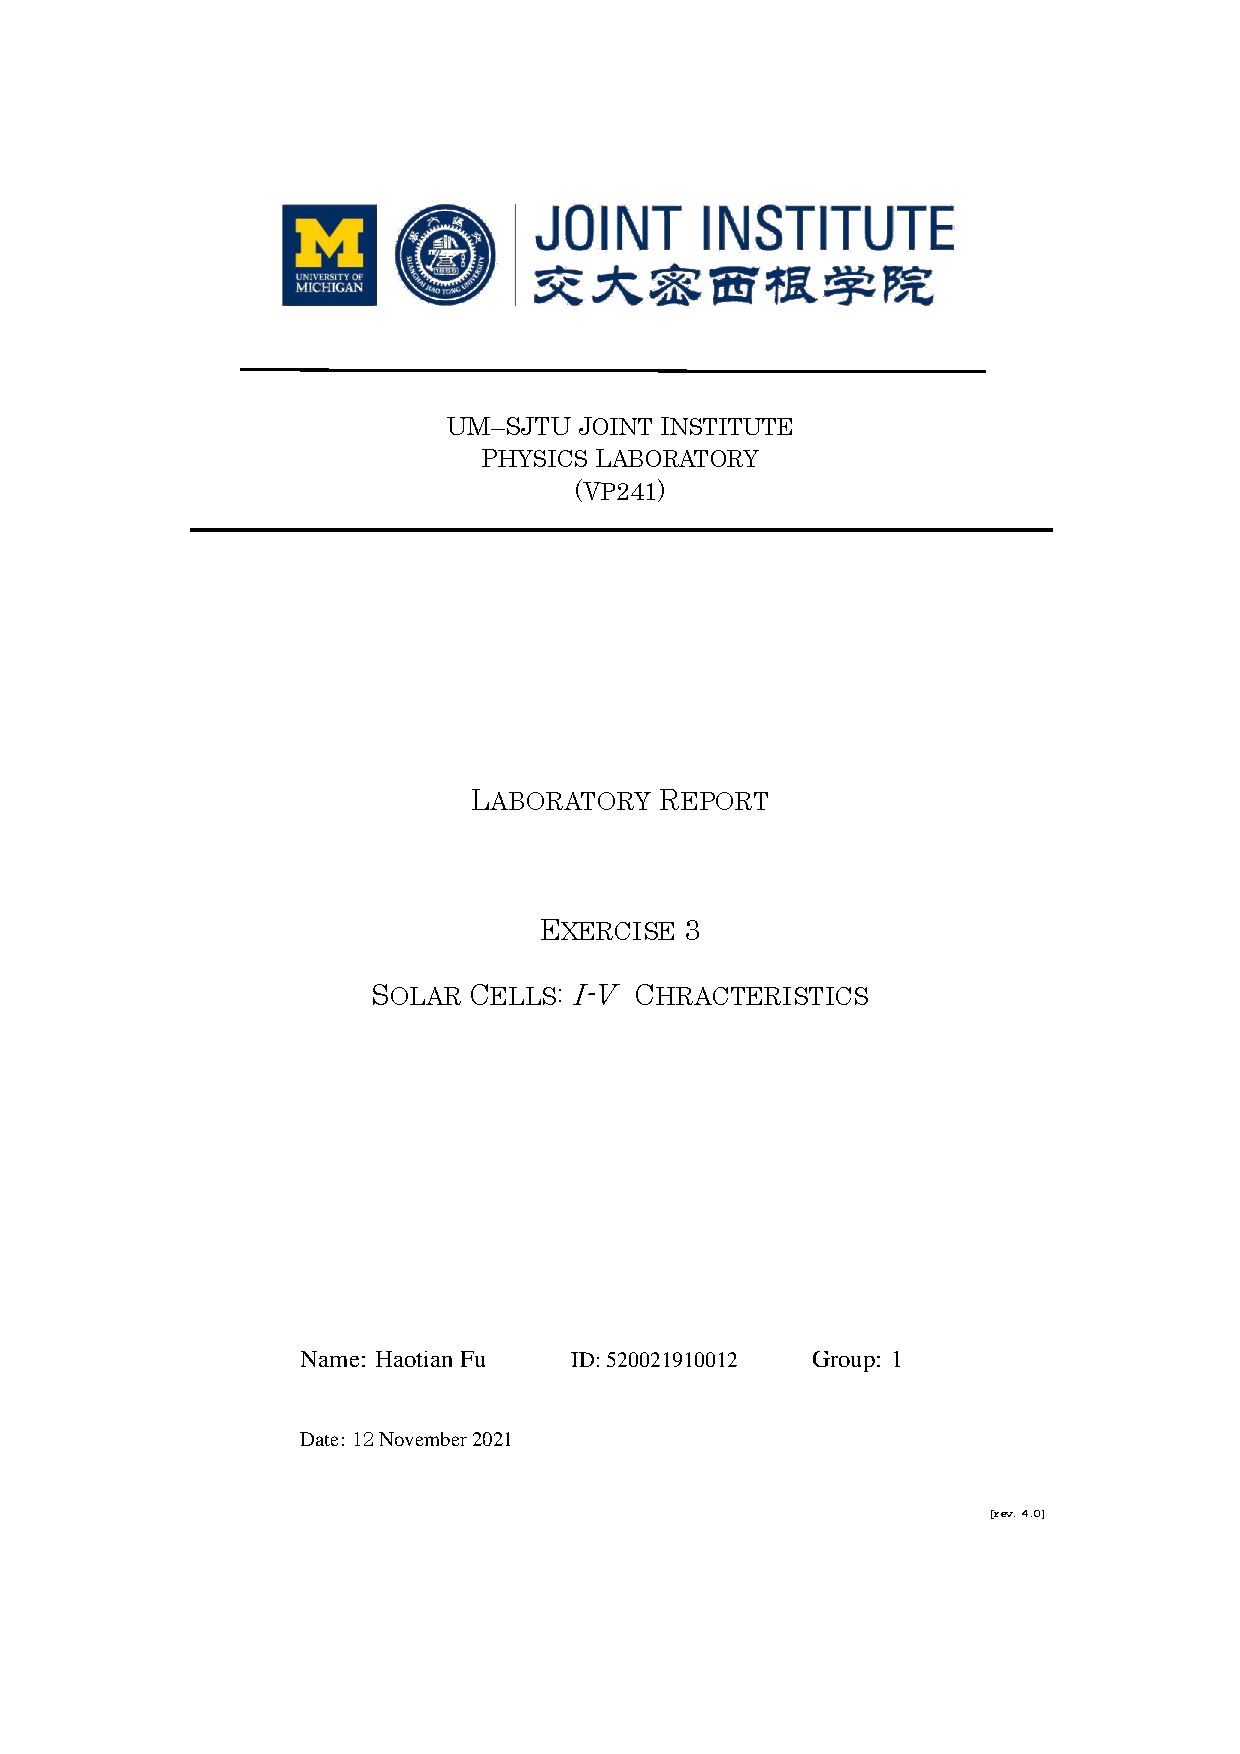
\includepdf{lab3_cover.pdf}

\newpage
\tableofcontents
\setcounter{page}{1}

\newpage
\listoffigures
\listoftables

\newpage
\section{Introduction}
The objective of this exercise is to urge students to be familiar with the working principle of a solar cell and study its current-voltage \textit{(I-V)} characteristics.

\subsection{Basic Concepts}
\begin{itemize}
	\item \textbf{Solar cell:}$^{[1]}$ Solar cells are devices which are able to directly transform solar radiation into electrical energy.
	      \begin{figure}[!htbp]
		      \centering
		      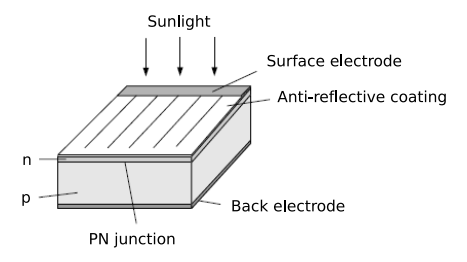
\includegraphics[width=0.45\textwidth]{solar_cell.png}
		      \caption{Solar cell}
	      \end{figure}
	\item \textbf{P-N junction:}$^{[2]}$ A p–n junction is a boundary or interface between two types of semiconductor materials, p-type and n-type, inside a single crystal of semiconductor.
	      \begin{figure}[!htbp]
		      \centering
		      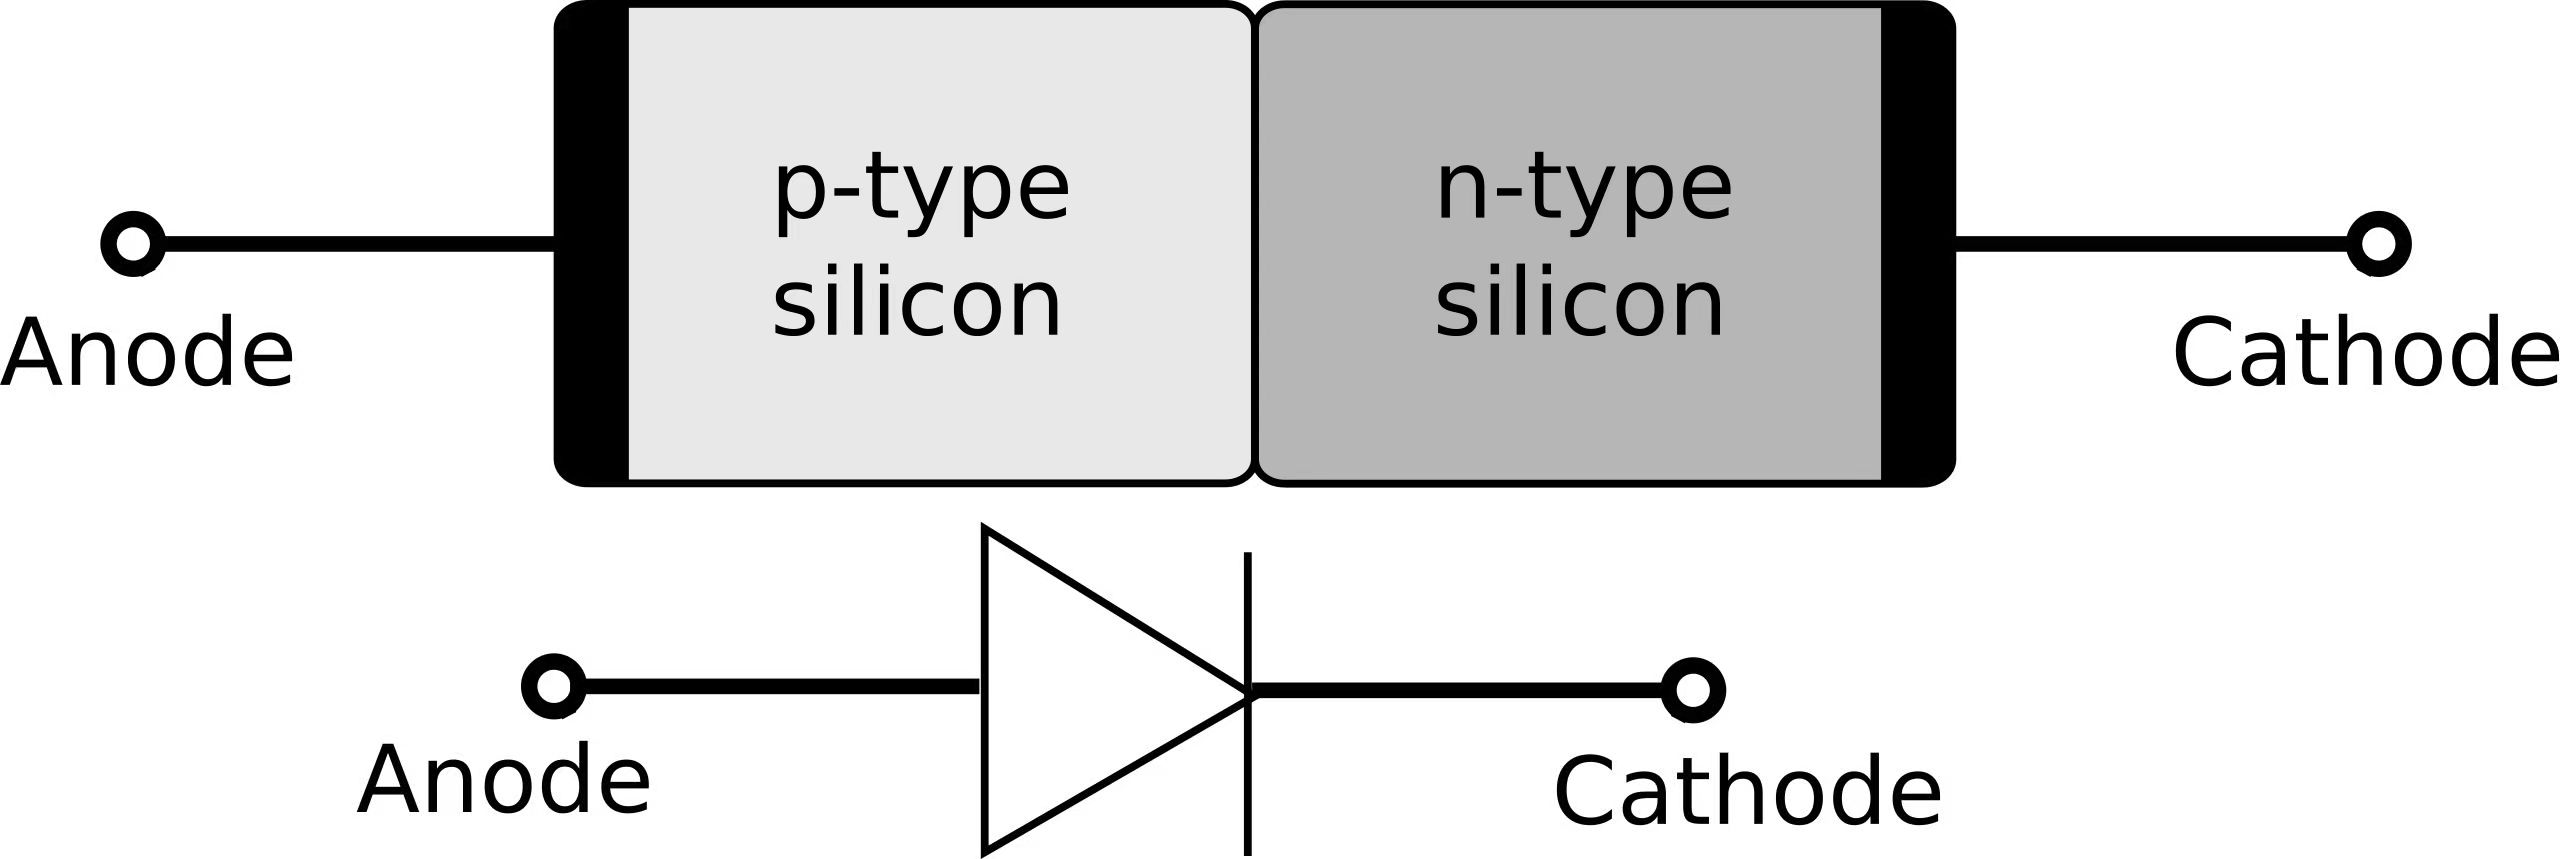
\includegraphics[width=0.4\textwidth]{pn_junction.jpg}
		      \caption{P-N junction}
	      \end{figure}
	\item \textbf{Photovoltaic (PV) effect:}$^{[3]}$ Photovoltaic (PV) effect is a process by which PV cell converts the absorbed sunlight energy into electricity.
	      \begin{figure}[!htbp]
		      \centering
		      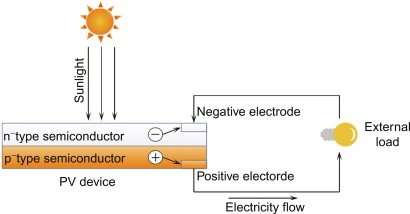
\includegraphics[width=0.5\textwidth]{photovoltaic_effect.jpg}
		      \caption{Photovoltaic effect}
	      \end{figure}
	\item \textbf{Fill factor:} Fill factor is the available power at the maximum power point ($P_\text{m}$) divided by the open circuit voltage ($V_\text{OC}$) and the short circuit current ($I_{\text{sc}}$).
	      \begin{equation}
		      F F=\frac{P_{\mathrm{m}}}{V_{\mathrm{oc}} I_{\mathrm{sc}}}=\frac{V_{\mathrm{m}} I_{\mathrm{m}}}{V_{\mathrm{oc}} I_{\mathrm{sc}}}
	      \end{equation}
	\item \textbf{Solar cell energy conversion efficiency:} The solar cell energy conversion efficiency $\eta$ is defined as
	      \begin{equation}
		      \eta=\frac{P_{\mathrm{m}}}{P_{\text {in }}} \times 100 \%
		      \label{eq::eta}
	      \end{equation}
	      where $P_{\text {in }}$ denotes the total radiant power incident on the solar cell while $P_\text{m}$ denotes the maximum output power.
\end{itemize}

\subsection{Theoretical Basis}
\subsubsection{The Principle of the Photovoltaic Effect$^{[1]}$}
\par When the light enters the $p-n$ junction near the solar cell surface, and the energy of
incident photons is greater than the forbidden bandwidth (energy gap) $E_g$, the incident
photons are absorbed and excite electron-hole pairs. Minority charge carriers in the $n-$ or
$p-$type area diffuse due to their density gradient. Some of them are able to diffuse to the
region of the $p-n$ junction where a built-in electric field exists. This field is directed from
the $n-$type to the $p-$type area. The minority carriers diffusing to the $p-n$ junction zone
between the $n-$type area and the $p-$type area are drawn by this electric field to the $p-$type
area (in case of the holes), or to the n-type area (in case of the electrons). This results in
an increase of positive charge accumulated in the p-type area and negative charge in the
$n-$type area. Consequently, a photoelectric potential difference is generated.


\subsubsection{Solar Cell Parameters}
\par The net current $I$ is
\begin{equation}
	I=I_{\mathrm{ph}}-I_{\mathrm{D}}=I_{\mathrm{ph}}-I_{0}\left[\exp \left(\frac{q V_{\mathrm{D}}}{n k_{\mathrm{B}} T}\right)-1\right]
	\label{eq::I}
\end{equation}
where $I_{\text{ph}}$ is the current from the $n-$type area to the $p-$area when there is light incident on the solar cell and $I_D$ is a forward diode current from the $p-$type to the $n-$type area, opposite to $I_{\text{ph}}$.
$V_D$ is the junction voltage, $I_0$ is the diode inverse saturation current, the coefficient $n$ is a theoretical coefficient, with its values ranging from 1 to 2, that characterizes the $p-n$ junction.
Furthermore, $q$ denotes the electron’s charge, $k_B$ is the Boltzmann’s constant, and $T$ is the temperature in the absolute (Kelvin) scale.

Ignoring the internal series resistance $R_s$, the voltage $V_D$ equals the terminal voltage $V$ and Eq.(\ref{eq::I}) can be rewritten as
\begin{equation}
	I=I_{\mathrm{ph}} - I_{0} \left[ \exp \left( \frac{q V}{n k_{\mathrm{B}} T}\right) - 1 \right]
	\label{eq::I_2}
\end{equation}

When the output is short, $i.e.$, $V=0$, the short-circuit current is
$$
	I_{\mathrm{sc}}=I_{\mathrm{ph}}
$$

whereas when the output is open, $i.e.$, $I=0$, the open-circuit voltage is
\begin{equation}
	V_{\mathrm{oc}}=\frac{n k_{\mathrm{B}} T}{q} \ln \left(\frac{I_{\mathrm{sc}}}{I_{0}}+1\right)
	\label{eq::V_OC}
\end{equation}

\subsubsection{Theoretical Graph}
\par Considering Eq.(\ref{eq::I_2}) and Eq.(\ref{eq::V_OC}), the corresponding $I-V$ characteristics curve is shown in Fig.(\ref{fig::theoretical_curve})
\begin{figure}[!htbp]
	\centering
	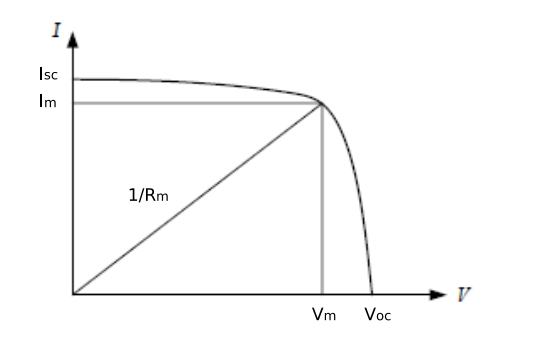
\includegraphics[width=0.6\textwidth]{theoretical_curve.png}
	\caption{The current-voltage characteristics of a solar cell.}
	\label{fig::theoretical_curve}
\end{figure}

\subsubsection{Solar Cell Equivalent Circuit}
\par As shown in Fig.(\ref{fig::equivalent_circuit}) , a solar cell can be thought of as composed of a $p-n$ junction diode $D$ and a constant current source $I_{\mathrm{ph}}$. Along with a series resistance $R_{\mathrm{s}}$ due to the electrodes in the solar cell and a parallel resistance $R_{\mathrm{sh}}$, all elements form a circuit equivalent to a $p$ - $n$ junction leak-circuit. For the equivalent circuit one can find the following relationship between the current and the voltage
$$
	I=I_{\mathrm{ph}}-I_{0}\left\{\exp \left[\frac{q\left(V+R_{\mathrm{s}} I\right)}{n k_{\mathrm{B}} T}\right]-1\right\}-\frac{V+R_{\mathrm{s}} I}{R_{\mathrm{sh}}}
$$
\begin{figure}[!htbp]
	\centering
	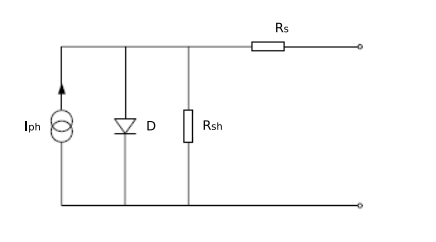
\includegraphics[width=0.5\textwidth]{equivalent_circuit.png}
	\caption{Solar cell equivalent circuit.}
	\label{fig::equivalent_circuit}
\end{figure}

\section{Apparatus and Measurement Procedure}

\subsection{Apparatus}
The setup consists of a photovoltaic device (5 W), a 300 W tungsten-halogen lamp
serving as a radiation source, two digital multimeters, two adjustable resistors, a solar
power meter, a wiring board and a measuring tape.

The precisions of the devices are shown in Table \ref{table::Multimeter_Precision}.
\begin{table}[htbp]
	\centering
	\begin{tabular}{cc}
		\hline
		Instrument  & Uncertainties          \\
		\hline
		DC Voltage  & $\pm (0.5\%+0.01)\,$V  \\
		DC Current  & $\pm (1.5\% + 0.1\,$mA \\
		Distance    & $\pm 0.1\%\,$cm        \\
		Solar power & $\pm 10\,$W/cm$^2$     \\
		\hline
	\end{tabular}
	\caption{Information of measurement instruments.}
	\label{table::Multimeter_Precision}
\end{table}

\subsection{Measurement Procedure}

In this exercise, the characteristics of four configurations of the solar cell are studied. For each configuration, the $I-V$ $P-V$, $P-R$ relations are studied and for each single configurations, the information about fill factor and energy conversion efficiency are also explored.
\begin{enumerate}
	\item Turn on both the light and the fan and then wait until the light reaches its working intensity.
	\item Design a measuring circuit with the photovoltaic device, multimeters set in an appropriate range, and the resistance. Connect the elements into a circuit using the provided wiring board.
	\item Adjust the distance between the light source and the photovoltaic device until the $V_\text{oc}$ and $I_\text{sc}$ of the two devices are about the same. Measure the solar power by the provided solar power meter.
	\item Change the distance between the light source and the photovoltaic device and measure the $I-V$ characteristics curves and the values of $V_\text{oc}$ and $I_\text{sc}$ in a single-device configuration. Measure the solar power at this distance.
	\item Plot
\end{enumerate}

\subsection{Safety Notice}

\begin{itemize}
	\item The temperature of the light source is very high, do not touch the cover.
	\item The power supply voltage of the light source is 220 V, beware of electric shock.
\end{itemize}


\section{Experimental Results}

First, we need to clarify the area we measured since the energy provided is closely related to the area of solar cells.
Corresponding data is as follows.

\begin{table}[H]
	\centering
	\begin{tabular}{cc}
		\hline
		length [cm] & width [cm] \\ \hline
		21.00       & 26.10      \\ \hline
	\end{tabular}
	\caption{Measurement data for area}
	\label{table::area}
\end{table}

\subsection{$I-V$ Characteristics}

The measurement data for $U$ and $I$ under different conditions are shown in Table \ref{table::126.0}.

\begin{table}[H]
	\centering
	\begin{tabular}{ccc||cc}
		\hline
		   & \multicolumn{2}{c||}{Series} & \multicolumn{2}{c}{Parallel}                                                               \\
		   & $U$ $\pm$ (0.5\% + 0.01) [V] & $I$ $\pm$ (1.5\% + 0.1) [mA] & $U$ $\pm$ (0.5\% + 0.01) [V] & $I$ $\pm$ (1.5\% + 0.1) [mA] \\
		\hline
		1  & 1.89  $\pm$ 0.02             & 43.5   $\pm$ 0.8             & 0.61   $\pm$ 0.013           & 90.5 $\pm$ 1.5               \\
		2  & 2.67  $\pm$ 0.03             & 43.2   $\pm$ 0.8             & 1.17   $\pm$ 0.016           & 88.0 $\pm$ 1.5               \\
		3  & 3.45  $\pm$ 0.03             & 42.1   $\pm$ 0.8             & 1.45   $\pm$ 0.018           & 87.0 $\pm$ 1.4               \\
		4  & 4.82  $\pm$ 0.04             & 40.7   $\pm$ 0.8             & 1.71   $\pm$ 0.019           & 85.6 $\pm$ 1.4               \\
		5  & 6.77  $\pm$ 0.05             & 39.3   $\pm$ 0.7             & 2.14   $\pm$ 0.02            & 83.8 $\pm$ 1.4               \\
		6  & 7.55  $\pm$ 0.05             & 38.4   $\pm$ 0.7             & 2.43   $\pm$ 0.03            & 82.4 $\pm$ 1.4               \\
		7  & 8.44  $\pm$ 0.06             & 37.1   $\pm$ 0.7             & 2.97   $\pm$ 0.03            & 79.7 $\pm$ 1.3               \\
		8  & 8.82  $\pm$ 0.06             & 35.6   $\pm$ 0.7             & 3.28   $\pm$ 0.03            & 78.2 $\pm$ 1.3               \\
		9  & 9.60  $\pm$ 0.06             & 34.3   $\pm$ 0.7             & 3.56   $\pm$ 0.03            & 76.5 $\pm$ 1.3               \\
		10 & 10.53 $\pm$ 0.07             & 32.0   $\pm$ 0.6             & 4.02   $\pm$ 0.03            & 73.9 $\pm$ 1.2               \\
		11 & 3.09  $\pm$ 0.03             & 43.0   $\pm$ 0.8             & 4.40   $\pm$ 0.03            & 71.3 $\pm$ 1.2               \\
		12 & 4.08  $\pm$ 0.03             & 42.0   $\pm$ 0.8             & 4.83   $\pm$ 0.04            & 67.7 $\pm$ 1.2               \\
		13 & 5.53  $\pm$ 0.04             & 40.5   $\pm$ 0.7             & 5.15   $\pm$ 0.04            & 64.4 $\pm$ 1.1               \\
		14 & 9.16  $\pm$ 0.06             & 35.4   $\pm$ 0.7             & 5.45   $\pm$ 0.04            & 61.2 $\pm$ 1.0               \\
		15 & 11.44 $\pm$ 0.07             & 28.6   $\pm$ 0.6             & 5.76   $\pm$ 0.04            & 57.6 $\pm$ 1.0               \\
		16 & 11.15 $\pm$ 0.07             & 29.5   $\pm$ 0.6             & 6.09   $\pm$ 0.04            & 53.3 $\pm$ 0.9               \\
		17 & 11.54 $\pm$ 0.07             & 28.9   $\pm$ 0.6             & 6.44   $\pm$ 0.05            & 47.9 $\pm$ 0.9               \\
		18 & 12.00 $\pm$ 0.07             & 26.7   $\pm$ 0.5             & 6.75   $\pm$ 0.05            & 42.4 $\pm$ 0.8               \\
		19 & 12.71 $\pm$ 0.08             & 24.2   $\pm$ 0.5             & 6.92   $\pm$ 0.05            & 38.8 $\pm$ 0.7               \\
		20 & 13.13 $\pm$ 0.08             & 22.4   $\pm$ 0.5             & 7.38   $\pm$ 0.05            & 27.8 $\pm$ 0.6               \\
		21 & 13.51 $\pm$ 0.08             & 20.7   $\pm$ 0.5             & 7.15   $\pm$ 0.06            & 33.4 $\pm$ 0.6               \\
		22 & 13.97 $\pm$ 0.08             & 18.3   $\pm$ 0.4             & 7.53   $\pm$ 0.05            & 23.5 $\pm$ 0.5               \\
		23 & 14.35 $\pm$ 0.09             & 16.2   $\pm$ 0.4             & 7.68   $\pm$ 0.05            & 19.1 $\pm$ 0.4               \\
		24 & 14.43 $\pm$ 0.09             & 15.6   $\pm$ 0.4             & 7.85   $\pm$ 0.05            & 13.9 $\pm$ 0.3               \\
		25 & 14.61 $\pm$ 0.09             & 14.6   $\pm$ 0.4             & 7.98   $\pm$ 0.05            & 9.3  $\pm$ 0.3               \\
		\hline
	\end{tabular}
	\caption{Measurement data for the $U$ vs. $I$ relation (series/parallel configuration).}
	\label{table::126.0}
\end{table}

\begin{table}[H]
	\centering
	\begin{tabular}{ccc||cc}
		\hline
		   & \multicolumn{2}{c||}{100 cm} & \multicolumn{2}{c}{144 cm}                                                                                       \\
		\hline
		   & $U$ $\pm$ (0.5\% + 0.01) [V] & $I$ $\pm$ (1.5\% + 0.1) [mA]           & $U$ $\pm$ (0.5\% + 0.01) [V]             & $I$ $\pm$ (1.5\% + 0.1) [mA] \\
		\hline
		1  & 9.15 $\pm$ 0.06              & 9.3                          $\pm$ 0.2 & 0.470$^*$                         $\pm$ 0.012 & 36.9 $\pm$ 0.7               \\
		2  & 9.09 $\pm$ 0.06              & 11.1                         $\pm$ 0.3 & 0.890$^*$                         $\pm$ 0.014 & 36.4 $\pm$ 0.6               \\
		3  & 9.00 $\pm$ 0.06              & 13.8                         $\pm$ 0.3 & 1.390$^*$                         $\pm$ 0.017 & 35.8 $\pm$ 0.6               \\
		4  & 8.94 $\pm$ 0.05              & 15.7                         $\pm$ 0.3 & 1.810$^*$                         $\pm$ 0.019 & 35.1 $\pm$ 0.6               \\
		5  & 8.86 $\pm$ 0.05              & 17.9                         $\pm$ 0.4 & 2.16                         $\pm$ 0.02  & 34.5 $\pm$ 0.6               \\
		6  & 8.80 $\pm$ 0.05              & 19.7                         $\pm$ 0.4 & 2.92                         $\pm$ 0.02  & 33.0 $\pm$ 0.6               \\
		7  & 8.65 $\pm$ 0.05              & 23.5                         $\pm$ 0.5 & 3.38                         $\pm$ 0.03  & 32.3 $\pm$ 0.6               \\
		8  & 8.46 $\pm$ 0.05              & 27.5                         $\pm$ 0.5 & 3.71                         $\pm$ 0.03  & 31.6 $\pm$ 0.6               \\
		9  & 8.33 $\pm$ 0.05              & 30.1                         $\pm$ 0.6 & 4.21                         $\pm$ 0.03  & 30.7 $\pm$ 0.6               \\
		10 & 8.21 $\pm$ 0.05              & 32.2                         $\pm$ 0.6 & 4.63                         $\pm$ 0.03  & 29.8 $\pm$ 0.5               \\
		11 & 8.07 $\pm$ 0.05              & 34.4                         $\pm$ 0.6 & 5.01                         $\pm$ 0.04  & 29.1 $\pm$ 0.5               \\
		12 & 7.92 $\pm$ 0.05              & 36.5                         $\pm$ 0.6 & 5.44                         $\pm$ 0.04  & 28.2 $\pm$ 0.5               \\
		13 & 7.75 $\pm$ 0.05              & 38.8                         $\pm$ 0.7 & 5.75                         $\pm$ 0.04  & 27.0 $\pm$ 0.5               \\
		14 & 7.59 $\pm$ 0.05              & 40.5                         $\pm$ 0.7 & 6.09                         $\pm$ 0.04  & 25.2 $\pm$ 0.5               \\
		15 & 7.37 $\pm$ 0.05              & 42.6                         $\pm$ 0.7 & 6.46                         $\pm$ 0.04  & 23.0 $\pm$ 0.4               \\
		16 & 6.71 $\pm$ 0.04              & 48.2                         $\pm$ 0.8 & 6.71                         $\pm$ 0.04  & 21.1 $\pm$ 0.4               \\
		17 & 6.22 $\pm$ 0.04              & 50.7                         $\pm$ 0.9 & 6.96                         $\pm$ 0.04  & 19.1 $\pm$ 0.4               \\
		18 & 5.52 $\pm$ 0.04              & 53.7                         $\pm$ 0.9 & 7.08                         $\pm$ 0.05  & 18.0 $\pm$ 0.4               \\
		19 & 5.21 $\pm$ 0.04              & 54.8                         $\pm$ 0.9 & 7.24                         $\pm$ 0.05  & 16.4 $\pm$ 0.3               \\
		20 & 4.77 $\pm$ 0.03              & 56.1                         $\pm$ 0.9 & 7.38                         $\pm$ 0.05  & 14.9 $\pm$ 0.3               \\
		21 & 4.58 $\pm$ 0.03              & 57.1                         $\pm$ 1.0 & 7.51                         $\pm$ 0.05  & 13.6 $\pm$ 0.3               \\
		22 & 3.61 $\pm$ 0.03              & 60.7                         $\pm$ 1.0 & 7.68                         $\pm$ 0.05  & 11.6 $\pm$ 0.3               \\
		23 & 2.97 $\pm$ 0.02              & 62.2                         $\pm$ 1.0 & 7.72                         $\pm$ 0.05  & 11.0 $\pm$ 0.3               \\
		24 & 1.690$^*$ $\pm$ 0.018             & 64.7                         $\pm$ 1.1 & 7.80                         $\pm$ 0.05  & 9.8  $\pm$ 0.2               \\
		25 & 1.040$^*$ $\pm$ 0.015             & 66.0                         $\pm$ 1.1 & 7.90                         $\pm$ 0.05  & 8.6  $\pm$ 0.2               \\
		\hline
	\end{tabular}
	\caption{Measurement data for the $U$ vs. $I$ relation (100 cm/144 cm configuration).}
	\label{table::100_144}
\end{table}

*\footnote{\textit{The star(*) here is to say the last 0 does not actually exist but due to the decimal number of uncertainty.}}

\begin{figure}[H]
	\centering
	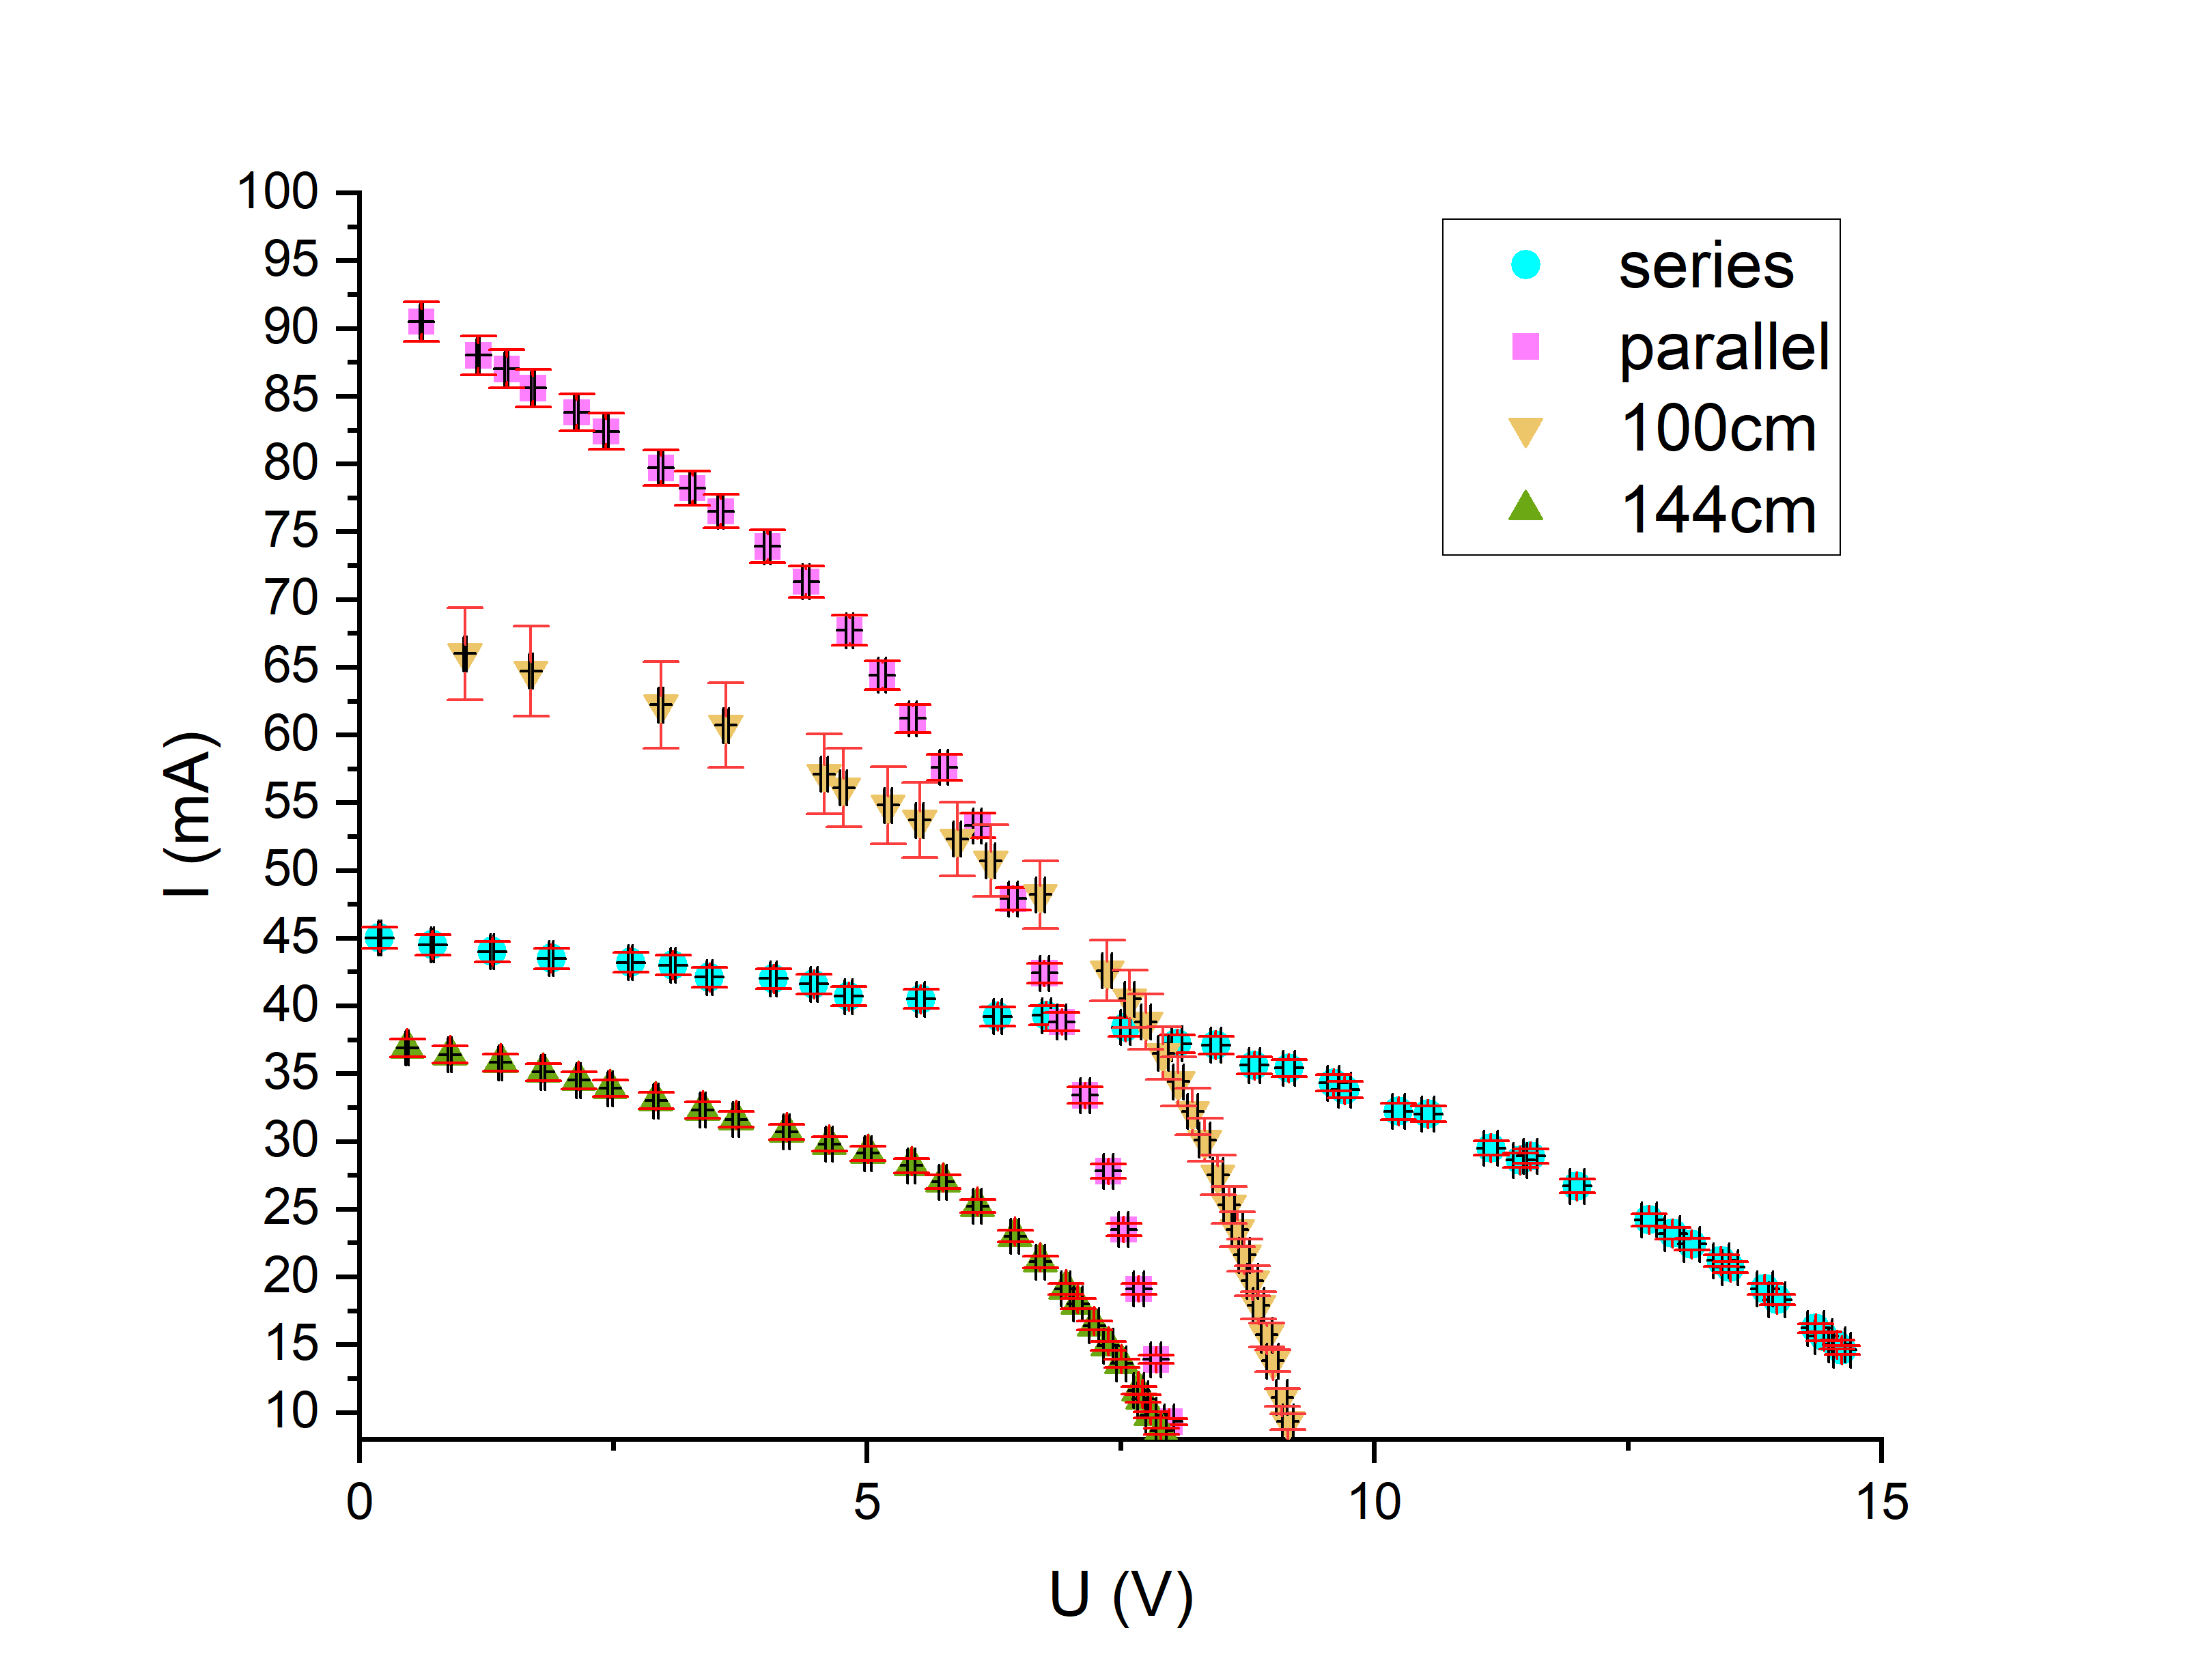
\includegraphics[width=0.8\textwidth]{I-V characteristic.png}
	\caption{$I-V$ characteristic curves of each configuration.}
	\label{fig::I-V}
\end{figure}

\subsection{$P-V$ Characteristics}

Here we try to plot the characteristics graph of $P-V$ relation.

The power of the solar cell is calculated as the product of $V$ and $I$. Take the first set of data as an example,
$$P = VI = 1.89 \times 43.5 \times 10^{-3} = 0.082 \pm 0.002\,\,\text{W}.$$

Perform simialr calculation for each set of data, the results are presented in Table \ref{table::P-U_1} and Table \ref{table::P-U_2}.

\begin{table}[H]
	\centering
	\begin{tabular}{c||cc|cc}
		\hline
		   & \multicolumn{2}{c|}{Series}  & \multicolumn{2}{c}{Parallel}                                                      \\
		   & $U$ $\pm$ (0.5\% + 0.01) [V] & $P$ [W]                      & $U$ $\pm$ (0.5\% + 0.01) [V] & $P$ [W]             \\
		\hline
		1  & 1.89  $\pm$ 0.02             & 0.082  $\pm$ 0.002           & 0.610$^*$   $\pm$ 0.013           & 0.0552 $\pm$ 0.0015 \\
		2  & 2.67  $\pm$ 0.03             & 0.115  $\pm$ 0.002           & 1.170$^*$   $\pm$ 0.016           & 0.103  $\pm$ 0.002  \\
		3  & 3.45  $\pm$ 0.03             & 0.145  $\pm$ 0.003           & 1.450$^*$   $\pm$ 0.018           & 0.126  $\pm$ 0.003  \\
		4  & 4.82  $\pm$ 0.04             & 0.196  $\pm$ 0.004           & 1.710$^*$   $\pm$ 0.019           & 0.146  $\pm$ 0.003  \\
		5  & 6.77  $\pm$ 0.05             & 0.266  $\pm$ 0.005           & 2.14   $\pm$ 0.02            & 0.179  $\pm$ 0.003  \\
		6  & 7.55  $\pm$ 0.05             & 0.290  $\pm$ 0.005           & 2.43   $\pm$ 0.03            & 0.200  $\pm$ 0.004  \\
		7  & 8.44  $\pm$ 0.06             & 0.313  $\pm$ 0.006           & 2.97   $\pm$ 0.03            & 0.237  $\pm$ 0.004  \\
		8  & 8.82  $\pm$ 0.06             & 0.314  $\pm$ 0.006           & 3.28   $\pm$ 0.03            & 0.256  $\pm$ 0.005  \\
		9  & 9.60  $\pm$ 0.06             & 0.329  $\pm$ 0.006           & 3.56   $\pm$ 0.03            & 0.272  $\pm$ 0.005  \\
		10 & 10.53 $\pm$ 0.07             & 0.337  $\pm$ 0.006           & 4.02   $\pm$ 0.03            & 0.297  $\pm$ 0.005  \\
		11 & 3.09  $\pm$ 0.03             & 0.133  $\pm$ 0.003           & 4.40   $\pm$ 0.03            & 0.314  $\pm$ 0.006  \\
		12 & 4.08  $\pm$ 0.03             & 0.171  $\pm$ 0.003           & 4.83   $\pm$ 0.04            & 0.327  $\pm$ 0.006  \\
		13 & 5.53  $\pm$ 0.04             & 0.224  $\pm$ 0.004           & 5.15   $\pm$ 0.04            & 0.332  $\pm$ 0.006  \\
		14 & 9.16  $\pm$ 0.06             & 0.324  $\pm$ 0.006           & 5.45   $\pm$ 0.04            & 0.334  $\pm$ 0.006  \\
		15 & 11.44 $\pm$ 0.07             & 0.327  $\pm$ 0.006           & 5.76   $\pm$ 0.04            & 0.332  $\pm$ 0.006  \\
		16 & 11.15 $\pm$ 0.07             & 0.329  $\pm$ 0.006           & 6.09   $\pm$ 0.04            & 0.325  $\pm$ 0.006  \\
		17 & 11.54 $\pm$ 0.07             & 0.334  $\pm$ 0.006           & 6.44   $\pm$ 0.05            & 0.308  $\pm$ 0.006  \\
		18 & 12.00 $\pm$ 0.07             & 0.320  $\pm$ 0.006           & 6.75   $\pm$ 0.05            & 0.286  $\pm$ 0.005  \\
		19 & 12.71 $\pm$ 0.08             & 0.308  $\pm$ 0.006           & 6.92   $\pm$ 0.05            & 0.268  $\pm$ 0.005  \\
		20 & 13.13 $\pm$ 0.08             & 0.294  $\pm$ 0.006           & 7.38   $\pm$ 0.05            & 0.205  $\pm$ 0.004  \\
		21 & 13.51 $\pm$ 0.08             & 0.280  $\pm$ 0.006           & 7.15   $\pm$ 0.06            & 0.239  $\pm$ 0.005  \\
		22 & 13.97 $\pm$ 0.08             & 0.256  $\pm$ 0.005           & 7.53   $\pm$ 0.05            & 0.177  $\pm$ 0.004  \\
		23 & 14.35 $\pm$ 0.09             & 0.232  $\pm$ 0.005           & 7.68   $\pm$ 0.05            & 0.147  $\pm$ 0.003  \\
		24 & 14.43 $\pm$ 0.09             & 0.225  $\pm$ 0.005           & 7.85   $\pm$ 0.05            & 0.109  $\pm$ 0.003  \\
		25 & 14.61 $\pm$ 0.09             & 0.213  $\pm$ 0.005           & 7.98   $\pm$ 0.05            & 0.074  $\pm$ 0.002  \\
		\hline
	\end{tabular}
	\caption{Power $P$ and uncertainty for four configurations.}
	\label{table::P-U_1}
\end{table}

*\footnote{\textit{The star(*) here is to say the last 0 does not actually exist but due to the decimal number of uncertainty.}}

\begin{figure}[H]
	\centering
	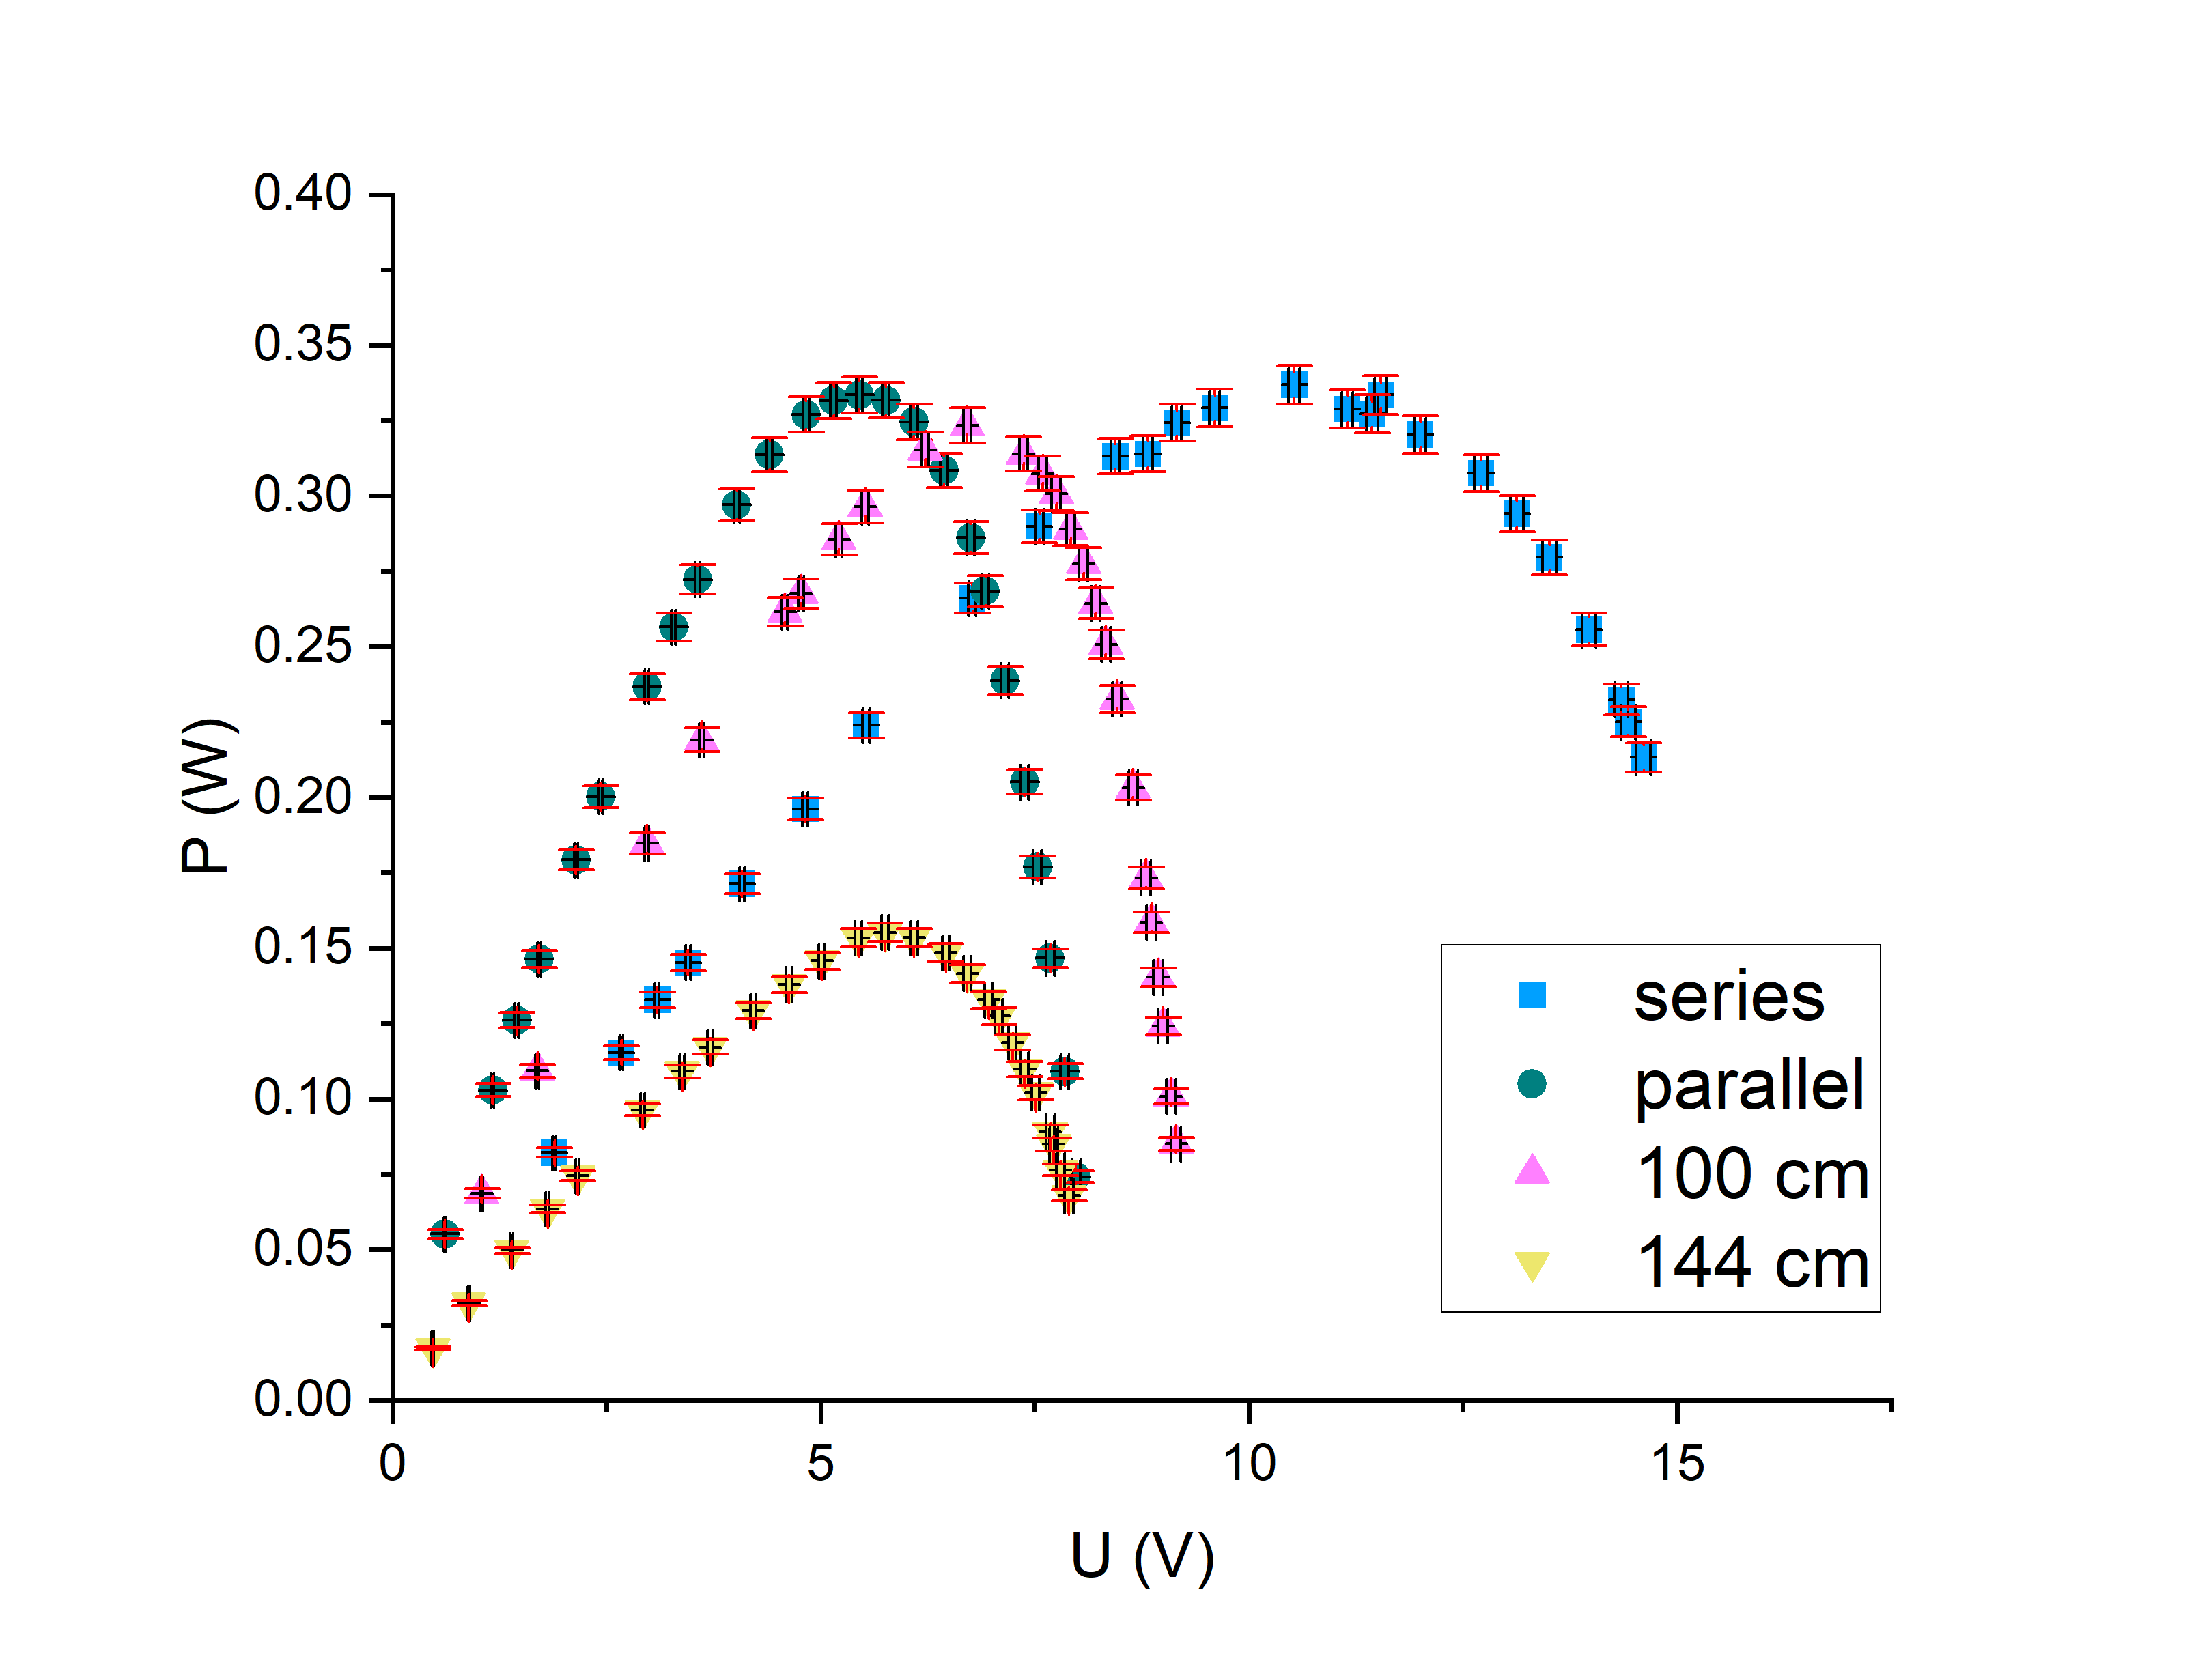
\includegraphics[width=0.8\textwidth]{P-U_characteristics.png}
	\caption{P-V characteristic curves of each configuration.}
	\label{fig::P-U}
\end{figure}

\begin{table}[H]
	\centering
	\begin{tabular}{c||cc|cc}
		\hline
		   & \multicolumn{2}{c|}{100 cm}  & \multicolumn{2}{c}{144 cm}                                                       \\
		   & $U$ $\pm$ (0.5\% + 0.01) [V] & $P$ [W]                    & $U$ $\pm$ (0.5\% + 0.01) [V] & $P$ [W]              \\
		\hline
		1  & 9.15  $\pm$ 0.06             & 0.085  $\pm$ 0.002         & 0.470$^*$   $\pm$ 0.012      & 0.0173  $\pm$ 0.0005 \\
		2  & 9.09  $\pm$ 0.06             & 0.101  $\pm$ 0.002         & 0.890$^*$   $\pm$ 0.014      & 0.0324  $\pm$ 0.0008 \\
		3  & 9.00  $\pm$ 0.06             & 0.124  $\pm$ 0.003         & 1.390$^*$   $\pm$ 0.017      & 0.0498  $\pm$ 0.0011 \\
		4  & 8.94  $\pm$ 0.05             & 0.140  $\pm$ 0.003         & 1.810$^*$   $\pm$ 0.019      & 0.0635  $\pm$ 0.0013 \\
		5  & 8.86  $\pm$ 0.05             & 0.159  $\pm$ 0.003         & 2.16   $\pm$ 0.02            & 0.075   $\pm$ 0.002  \\
		6  & 8.80  $\pm$ 0.05             & 0.173  $\pm$ 0.004         & 2.92   $\pm$ 0.02            & 0.096   $\pm$ 0.002  \\
		7  & 8.65  $\pm$ 0.05             & 0.203  $\pm$ 0.004         & 3.38   $\pm$ 0.03            & 0.109   $\pm$ 0.002  \\
		8  & 8.46  $\pm$ 0.05             & 0.233  $\pm$ 0.005         & 3.71   $\pm$ 0.03            & 0.117   $\pm$ 0.002  \\
		9  & 8.33  $\pm$ 0.05             & 0.251  $\pm$ 0.005         & 4.21   $\pm$ 0.03            & 0.129   $\pm$ 0.003  \\
		10 & 8.21  $\pm$ 0.05             & 0.264  $\pm$ 0.005         & 4.63   $\pm$ 0.03            & 0.138   $\pm$ 0.003  \\
		11 & 8.07  $\pm$ 0.05             & 0.278  $\pm$ 0.005         & 5.01   $\pm$ 0.04            & 0.146   $\pm$ 0.003  \\
		12 & 7.92  $\pm$ 0.05             & 0.289  $\pm$ 0.005         & 5.44   $\pm$ 0.04            & 0.153   $\pm$ 0.003  \\
		13 & 7.75  $\pm$ 0.05             & 0.301  $\pm$ 0.006         & 5.75   $\pm$ 0.04            & 0.155   $\pm$ 0.003  \\
		14 & 7.59  $\pm$ 0.05             & 0.307  $\pm$ 0.006         & 6.09   $\pm$ 0.04            & 0.153   $\pm$ 0.003  \\
		15 & 7.37  $\pm$ 0.05             & 0.314  $\pm$ 0.006         & 6.46   $\pm$ 0.04            & 0.149   $\pm$ 0.003  \\
		16 & 6.71  $\pm$ 0.04             & 0.323  $\pm$ 0.006         & 6.71   $\pm$ 0.04            & 0.142   $\pm$ 0.003  \\
		17 & 6.22  $\pm$ 0.04             & 0.315  $\pm$ 0.006         & 6.96   $\pm$ 0.04            & 0.133   $\pm$ 0.003  \\
		18 & 5.52  $\pm$ 0.04             & 0.296  $\pm$ 0.005         & 7.08   $\pm$ 0.05            & 0.127   $\pm$ 0.003  \\
		19 & 5.21  $\pm$ 0.04             & 0.286  $\pm$ 0.005         & 7.24   $\pm$ 0.05            & 0.119   $\pm$ 0.003  \\
		20 & 4.77  $\pm$ 0.03             & 0.268  $\pm$ 0.005         & 7.38   $\pm$ 0.05            & 0.110   $\pm$ 0.002  \\
		21 & 4.58  $\pm$ 0.03             & 0.262  $\pm$ 0.005         & 7.51   $\pm$ 0.05            & 0.102   $\pm$ 0.002  \\
		22 & 3.61  $\pm$ 0.03             & 0.219  $\pm$ 0.004         & 7.68   $\pm$ 0.05            & 0.089   $\pm$ 0.002  \\
		23 & 2.97  $\pm$ 0.02             & 0.185  $\pm$ 0.003         & 7.72   $\pm$ 0.05            & 0.085   $\pm$ 0.002  \\
		24 & 1.690$^*$  $\pm$ 0.018       & 0.109  $\pm$ 0.002         & 7.80   $\pm$ 0.05            & 0.076   $\pm$ 0.002  \\
		25 & 1.040$^*$  $\pm$ 0.015       & 0.0686 $\pm$ 0.0015        & 7.90   $\pm$ 0.05            & 0.068   $\pm$ 0.002  \\
		\hline
	\end{tabular}
	\caption{Power $P$ and uncertainty for four configurations.}
	\label{table::P-U_2}
\end{table}
*\footnote{\textit{The star(*) here is to say the last 0 does not actually exist but due to the decimal number of uncertainty.}}

\subsection{Other relavant data}

For $I_\text{sc}$ and $U_\text{oc}$, we measured the data listing as follows.

\begin{table}[H]
	\centering
	\begin{tabular}{ccc}
		\hline
		         & $U_\text{oc}$ [V] & $I_\text{sc}$ [mA] \\
		\hline
		126.0 cm & 8.69  $\pm$ 0.05  & 44.3 $\pm$ 0.8     \\
		95.8 cm  & 7.71  $\pm$ 0.05  & 46.5 $\pm$ 0.8     \\
		series   & 16.42 $\pm$ 0.09  & 45.1 $\pm$ 0.8     \\
		parallel & 8.21  $\pm$ 0.05  & 90.0 $\pm$ 1.5     \\
		\hline
	\end{tabular}
	\caption{Measurement data for $U_\text{oc}$ and $I_\text{sc}$.}
	\label{table:ocsc}
\end{table}

Here we will further report other data such as $R_\text{m}$, $P_\text{m}$, $FF$, and $\eta$.

The resistance of the external load are caluclated through Ohm's law $\displaystyle R = \frac{V}{I}$. Take the first set of data as an example,
$$R = \frac{V}{I} = \frac{1.89}{43.5\times 10^{-3}} = 43.4 \pm 0.9\,\,\Omega.$$

Perform simialr calculation for each set of data, the results are presented in Table \ref{table::R}

\begin{table}[H]
	\centering
	\begin{tabular}{c|cccc}
		\hline
		   & Series                                       & Parallel        & 100 cm         & 144 cm         \\
		   & \multicolumn{4}{c}{R $\pm$ $u_R$ [$\Omega$]}                                                     \\
		\hline
		1  & 43.4 $\pm$ 0.9                               & 6.7 $\pm$ 0.2   & 980 $\pm$ 30   & 12.7 $\pm$ 0.4 \\
		2  & 61.8 $\pm$ 1.2                               & 13.3 $\pm$ 0.3  & 820 $\pm$ 20   & 24.5 $\pm$ 0.6 \\
		3  & 81.9 $\pm$ 1.6                               & 16.7 $\pm$ 0.3  & 652 $\pm$ 15   & 38.8 $\pm$ 0.8 \\
		4  & 118 $\pm$ 2                                  & 20.0 $\pm$ 0.4  & 569 $\pm$ 13   & 51.6 $\pm$ 1.1 \\
		5  & 172 $\pm$ 3                                  & 25.5 $\pm$ 0.5  & 495 $\pm$ 11   & 62.6 $\pm$ 1.3 \\
		6  & 197 $\pm$ 4                                  & 29.5 $\pm$ 0.5  & 447 $\pm$ 9    & 88 $\pm$ 2     \\
		7  & 227 $\pm$ 4                                  & 37.3 $\pm$ 0.7  & 368 $\pm$ 7    & 105 $\pm$ 2    \\
		8  & 248 $\pm$ 5                                  & 41.9 $\pm$ 0.8  & 308 $\pm$ 6    & 117 $\pm$ 2    \\
		9  & 280 $\pm$ 5                                  & 46.5 $\pm$ 0.8  & 277 $\pm$ 5    & 137 $\pm$ 3    \\
		10 & 329 $\pm$ 6                                  & 54.4 $\pm$ 1.0  & 255 $\pm$ 5    & 155 $\pm$ 3    \\
		11 & 71.9 $\pm$ 1.4                               & 61.7 $\pm$ 1.1  & 235 $\pm$ 4    & 172 $\pm$ 3    \\
		12 & 97.1 $\pm$ 1.8                               & 71.3 $\pm$ 1.3  & 217 $\pm$ 4    & 193 $\pm$ 4    \\
		13 & 137 $\pm$ 3                                  & 80.0 $\pm$ 1.4  & 200 $\pm$ 4    & 213 $\pm$ 4    \\
		14 & 259 $\pm$ 5                                  & 89.1 $\pm$ 1.6  & 187 $\pm$ 3    & 242 $\pm$ 5    \\
		15 & 400 $\pm$ 8                                  & 100.0 $\pm$ 1.8 & 173 $\pm$ 3    & 281 $\pm$ 6    \\
		16 & 378 $\pm$ 7                                  & 114 $\pm$ 2     & 139 $\pm$ 3    & 318 $\pm$ 7    \\
		17 & 399 $\pm$ 8                                  & 134 $\pm$ 2     & 123 $\pm$ 2    & 364 $\pm$ 8    \\
		18 & 449 $\pm$ 9                                  & 159 $\pm$ 3     & 103 $\pm$ 2    & 393 $\pm$ 8    \\
		19 & 525 $\pm$ 10                                 & 178 $\pm$ 3     & 95 $\pm$ 2     & 441 $\pm$ 10   \\
		20 & 586 $\pm$ 12                                 & 265 $\pm$ 5     & 85 $\pm$ 2     & 495 $\pm$ 11   \\
		21 & 653 $\pm$ 13                                 & 214 $\pm$ 4     & 80.2 $\pm$ 1.5 & 552 $\pm$ 13   \\
		22 & 763 $\pm$ 16                                 & 320 $\pm$ 6     & 59.5 $\pm$ 1.1 & 662 $\pm$ 16   \\
		23 & 886 $\pm$ 19                                 & 402 $\pm$ 9     & 47.7 $\pm$ 0.9 & 702 $\pm$ 17   \\
		24 & 930 $\pm$ 20                                 & 565 $\pm$ 13    & 26.1 $\pm$ 0.5 & 796 $\pm$ 20   \\
		25 & 1000 $\pm$ 20                                & 860 $\pm$ 20    & 15.8 $\pm$ 0.3 & 920 $\pm$ 20   \\
		\hline
	\end{tabular}
	\caption{Resistance $R$ for the four configurations.}
	\label{table::R}
\end{table}

Conclude what we have derived so far, the maximum output power and the corresponding $V_\text{m}, I_\text{m}, R_\text{m}$ can be found by consulting Table \ref{table::P-U_1}, Table \ref{table::P-U_2}, and Table \ref{table::R}.
The results are presented in Table \ref{table::Pmax}.

\begin{table}[H]
	\centering
	\begin{tabular}{ccccc}
		\hline
		         & $U_\text{m}$ [V] & $I_\text{m}$ [mA] & $P_\text{m}$ [W]   & $R_\text{m}\,\,[\Omega]$ \\
		\hline
		Series   & 11.54 $\pm$ 0.07 & 28.9 $\pm$ 0.6    & 0.334  $\pm$ 0.006 & 399   $\pm$ 8            \\
		Parallel & 5.45  $\pm$ 0.04 & 61.2 $\pm$ 1.0    & 0.334  $\pm$ 0.006 & 89.1 $\pm$ 1.6           \\
		100.0 cm & 6.71  $\pm$ 0.04 & 48.2 $\pm$ 0.8    & 0.323  $\pm$ 0.006 & 139   $\pm$ 3            \\
		144.0 cm & 5.75  $\pm$ 0.04 & 29.1 $\pm$ 0.5    & 0.155  $\pm$ 0.003 & 213   $\pm$ 4            \\
		\hline
	\end{tabular}
	\caption{$V_\text{m}$, $I_\text{m}$ and $P_\text{m}$ in four configurations.}
	\label{table::Pmax}
\end{table}

The fill factor $FF$ can be then calculated out of Eq.(1). Take the 100.0 cm configuration as an example, (here we assume 100.0 cm shares the same data with 95.8 cm due to data missing)
$$FF = \frac{P_\text{m}}{U_\text{oc}I_\text{sc}} = \frac{0.334}{7.71\times 46.5\times 10^{-3}} = 0.932 \pm 0.019.$$

The fill factor of each single configuration are calculated as shown and the results are presented in Table \ref{table::fill factor}.

\begin{table}[H]
	\centering
	\begin{tabular}{cc}
		\hline
		          & $FF$               \\
		\hline
		144.0 cm  & 0.403  $\pm$ 0.011 \\
		100.0  cm & 0.932  $\pm$ 0.019 \\
		\hline
	\end{tabular}
	\caption{Fill factor of single configuration.}
	\label{table::fill factor}
\end{table}

The measurement data for the area are shown in Table \ref{table::area}. See this table at the beginning of this section.

The measurement result of power of six points on the board are shown in Table \ref{table::P_in}.
\begin{table}[H]
	\centering
	\begin{tabular}{ccccccc}
		\hline
		                                                       & 1   & 2     & 3     & 4     & 5     & 6   \\
		\hline
		$P_{100.0}\,\,[\text{W/m}^2] \pm 10\,\,[\text{W/m}^2]$ & 391 & 275   & 168   & 381   & 250   & 207 \\
		$P_{144.0}\,\,[\text{W/m}^2] \pm 10\,\,[\text{W/m}^2]$ & 169 & 108   & 112   & 161   & 110   & 111 \\
		$P_{126.0}\,\,[\text{W/m}^2] \pm 10\,\,[\text{W/m}^2]$ & 207 & 139   & 136   & 210   & 135   & 142 \\
		$P_{95.8} \,\,[\text{W/m}^2] \pm 10\,\,[\text{W/m}^2]$ & 203 & 192.5 & 174.3 & 163.0 & 159.2 & 243 \\
		\hline
	\end{tabular}
	\caption{Measurement data for solar power.}
	\label{table::P_in}
\end{table}

The average of the power per square meter is
$$\overline{P_{100.0}} = \frac{1}{6}(391+275+168+381+250+207) = (300 \pm 100)\,\,\text{W/m}^2,$$
$$\overline{P_{144.0}} = \frac{1}{6}(169+108+112+161+110+111) = (130 \pm 30)\,\,\text{W/m}^2.$$

The total power is
$$P_{\text{in},100.0} = \overline{P_{100.0}}L_1L_2 = 300 \times 0.2610 \times 0.2100 = 16 \pm 11\,\,\text{W},$$
$$P_{\text{in},144.0} = \overline{P_{144.0}}L_1L_2 = 130 \times 0.2610 \times 0.2100 = 7 \pm 5\,\,\text{W}.$$

The power energy conversion efficiency can then be calculated from Eq.(\ref{eq::eta}), as
$$\eta_{100.0} = \frac{P_\text{m}}{P_{\text{in},100.0}} \times 100\% = \frac{0.323}{16} \times 100\%= 2.0\% \pm 1.4\%,$$
$$\eta_{144.0} = \frac{P_\text{m}}{P_{\text{in},144.0}} \times 100\% = \frac{0.155}{7} \times 100\%= 2.2\% \pm 1.6\%,$$



\section{Uncertainty Analysis}

\subsection{$I-V$ Characteristics}

The uncertainty of $V$ is $0.5\%+0.01$ V, and the uncertainty of $I$ is $1.5\%+0.1$ mA. Take the first set of data as an example,
$$u_{V} = 0.5\% \times 1.89 + 0.01 = 0.02\,\text{V}.$$
$$u_{I} = 1.5\% \times 43.5 + 0.1 = 0.8\,\text{mA}.$$
All the uncertainties of $V$ and $I$ are calculated in this way and the results are shown in Table \ref{table::unI-V}.

\begin{table}[H]
	\centering
	\begin{tabular}{c|cc||cc||cc||cc}
		\hline
		   & \multicolumn{2}{c||}{Series} & \multicolumn{2}{c||}{Parallel} & \multicolumn{2}{c||}{100 cm} & \multicolumn{2}{c}{144 cm}                                                   \\
		\hline
		   & $u_V$ [V]                    & $u_I$ [mA]                     & $u_V$ [V]                    & $u_I$ [mA]                 & $u_V$ [V] & $u_I$ [mA] & $u_V$ [V] & $u_I$ [mA] \\
		\hline
		1  & 0.02                         & 0.8                            & 0.013                        & 1.5                        & 0.06      & 0.2        & 0.012     & 0.7        \\
		2  & 0.03                         & 0.8                            & 0.016                        & 1.5                        & 0.06      & 0.3        & 0.014     & 0.6        \\
		3  & 0.03                         & 0.8                            & 0.018                        & 1.4                        & 0.06      & 0.3        & 0.017     & 0.6        \\
		4  & 0.04                         & 0.8                            & 0.019                        & 1.4                        & 0.05      & 0.3        & 0.019     & 0.6        \\
		5  & 0.05                         & 0.7                            & 0.02                         & 1.4                        & 0.05      & 0.4        & 0.02      & 0.6        \\
		6  & 0.05                         & 0.7                            & 0.03                         & 1.4                        & 0.05      & 0.4        & 0.02      & 0.6        \\
		7  & 0.06                         & 0.7                            & 0.03                         & 1.3                        & 0.05      & 0.5        & 0.03      & 0.6        \\
		8  & 0.06                         & 0.7                            & 0.03                         & 1.3                        & 0.05      & 0.5        & 0.03      & 0.6        \\
		9  & 0.06                         & 0.7                            & 0.03                         & 1.3                        & 0.05      & 0.6        & 0.03      & 0.6        \\
		10 & 0.07                         & 0.6                            & 0.03                         & 1.2                        & 0.05      & 0.6        & 0.03      & 0.5        \\
		11 & 0.03                         & 0.8                            & 0.03                         & 1.2                        & 0.05      & 0.6        & 0.04      & 0.5        \\
		12 & 0.03                         & 0.8                            & 0.04                         & 1.2                        & 0.05      & 0.6        & 0.04      & 0.5        \\
		13 & 0.04                         & 0.7                            & 0.04                         & 1.1                        & 0.05      & 0.7        & 0.04      & 0.5        \\
		14 & 0.06                         & 0.7                            & 0.04                         & 1.0                        & 0.05      & 0.7        & 0.04      & 0.5        \\
		15 & 0.07                         & 0.6                            & 0.04                         & 1.0                        & 0.05      & 0.7        & 0.04      & 0.4        \\
		16 & 0.07                         & 0.6                            & 0.04                         & 0.9                        & 0.04      & 0.8        & 0.04      & 0.4        \\
		17 & 0.07                         & 0.6                            & 0.05                         & 0.9                        & 0.04      & 0.9        & 0.04      & 0.4        \\
		18 & 0.07                         & 0.5                            & 0.05                         & 0.8                        & 0.04      & 0.9        & 0.05      & 0.4        \\
		19 & 0.08                         & 0.5                            & 0.05                         & 0.7                        & 0.04      & 0.9        & 0.05      & 0.3        \\
		20 & 0.08                         & 0.5                            & 0.05                         & 0.6                        & 0.03      & 0.9        & 0.05      & 0.3        \\
		21 & 0.08                         & 0.5                            & 0.06                         & 0.6                        & 0.03      & 1.0        & 0.05      & 0.3        \\
		22 & 0.08                         & 0.4                            & 0.05                         & 0.5                        & 0.03      & 1.0        & 0.05      & 0.3        \\
		23 & 0.09                         & 0.4                            & 0.05                         & 0.4                        & 0.02      & 1.0        & 0.05      & 0.3        \\
		24 & 0.09                         & 0.4                            & 0.05                         & 0.3                        & 0.018     & 1.1        & 0.05      & 0.2        \\
		25 & 0.09                         & 0.4                            & 0.05                         & 0.3                        & 0.015     & 1.1        & 0.05      & 0.2        \\
		\hline
	\end{tabular}
	\caption{Uncertainty of the data for $I$-$V$ characteristic.}
	\label{table::unI-V}
\end{table}

\subsection{$P-V$ Characteristics}

For $P = VI$, its uncertainty is calculated as
$$u_P = \sqrt{(\frac{\partial P}{\partial V}u_V)^2 + (\frac{\partial P}{\partial I}u_I)^2} = \sqrt{(Iu_V)^2 + (Vu_I)^2}.$$

Take the first set of data as an example,
$$u_P = \sqrt{(Iu_V)^2 + (Vu_I)^2} = \sqrt{(43.5\times 10^{-3}\times 0.02)^2 + (1.89\times 0.8\times 10^{-3})^2} = 0.002\,\text{W}.$$

\begin{table}[H]\centering
	\begin{tabular}{c|cccc}
		\hline
		   & Series    & Parallel  & 100 cm    & 144 cm    \\
		   & $u_P$ [W] & $u_P$ [W] & $u_P$ [W] & $u_P$ [W] \\
		\hline
		1  & 0.002     & 0.0015    & 0.002     & 0.0005    \\
		2  & 0.002     & 0.002     & 0.002     & 0.0008    \\
		3  & 0.003     & 0.003     & 0.003     & 0.0011    \\
		4  & 0.004     & 0.003     & 0.003     & 0.0013    \\
		5  & 0.005     & 0.003     & 0.003     & 0.002     \\
		6  & 0.005     & 0.004     & 0.004     & 0.002     \\
		7  & 0.006     & 0.004     & 0.004     & 0.002     \\
		8  & 0.006     & 0.005     & 0.005     & 0.002     \\
		9  & 0.006     & 0.005     & 0.005     & 0.003     \\
		10 & 0.006     & 0.005     & 0.005     & 0.003     \\
		11 & 0.003     & 0.006     & 0.005     & 0.003     \\
		12 & 0.003     & 0.006     & 0.005     & 0.003     \\
		13 & 0.004     & 0.006     & 0.006     & 0.003     \\
		14 & 0.006     & 0.006     & 0.006     & 0.003     \\
		15 & 0.006     & 0.006     & 0.006     & 0.003     \\
		16 & 0.006     & 0.006     & 0.006     & 0.003     \\
		17 & 0.006     & 0.006     & 0.006     & 0.003     \\
		18 & 0.006     & 0.005     & 0.005     & 0.003     \\
		19 & 0.006     & 0.005     & 0.005     & 0.003     \\
		20 & 0.006     & 0.004     & 0.005     & 0.002     \\
		21 & 0.006     & 0.005     & 0.005     & 0.002     \\
		22 & 0.005     & 0.004     & 0.004     & 0.002     \\
		23 & 0.005     & 0.003     & 0.003     & 0.002     \\
		24 & 0.005     & 0.003     & 0.002     & 0.002     \\
		25 & 0.005     & 0.002     & 0.0015    & 0.002     \\
		\hline
	\end{tabular}
	\caption{Uncertainty of data for $P$.}
	\label{table::unP}
\end{table}


\subsection{Other relevant data}

\subsubsection{$R$}

For $R = \frac{V}{I}$, its uncertainty is calculated as
$$u_R = \sqrt{(\frac{\partial R}{\partial V}u_V)^2 + (\frac{\partial R}{\partial I}u_I)^2} = \sqrt{(\frac{u_V}{I})^2 + (-\frac{V}{I^2}u_I)^2}.$$

Take the first set of data as an example,
$$u_R = \sqrt{(\frac{u_U}{I})^2 + (-\frac{U}{I^2}u_I)^2} = \sqrt{(\frac{0.02}{43.5\times 10^{-3}})^2 + (-\frac{1.89}{43.5^2}\times 0.8)^2} = 0.9\,\Omega .$$

Perform simialr calculation for each set of data, the results are presented in Table \ref{table::unR}

\begin{table}[H]\centering
	\begin{tabular}{c|cccc}
		\hline
		   & Series                               & Parallel & 100 cm & 144 cm \\
		   & \multicolumn{4}{c}{$u_R$ [$\Omega$]}                              \\
		\hline
		1  & 0.9                                  & 0.2      & 30     & 0.4    \\
		2  & 1.2                                  & 0.3      & 20     & 0.6    \\
		3  & 1.6                                  & 0.3      & 15     & 0.8    \\
		4  & 2                                    & 0.4      & 13     & 1.1    \\
		5  & 3                                    & 0.5      & 11     & 1.3    \\
		6  & 4                                    & 0.5      & 9      & 2      \\
		7  & 4                                    & 0.7      & 7      & 2      \\
		8  & 5                                    & 0.8      & 6      & 2      \\
		9  & 5                                    & 0.8      & 5      & 3      \\
		10 & 6                                    & 1.0      & 5      & 3      \\
		11 & 1.4                                  & 1.1      & 4      & 3      \\
		12 & 1.8                                  & 1.3      & 4      & 4      \\
		13 & 3                                    & 1.4      & 4      & 4      \\
		14 & 5                                    & 1.6      & 3      & 5      \\
		15 & 8                                    & 1.8      & 3      & 6      \\
		16 & 7                                    & 2        & 3      & 7      \\
		17 & 8                                    & 2        & 2      & 8      \\
		18 & 9                                    & 3        & 2      & 8      \\
		19 & 10                                   & 3        & 2      & 10     \\
		20 & 12                                   & 5        & 2      & 11     \\
		21 & 13                                   & 4        & 1.5    & 13     \\
		22 & 16                                   & 6        & 1.1    & 16     \\
		23 & 19                                   & 9        & 0.9    & 17     \\
		24 & 20                                   & 13       & 0.5    & 20     \\
		25 & 20                                   & 20       & 0.3    & 20     \\
		\hline
	\end{tabular}
	\caption{Uncertainty of data for $R$.}
	\label{table::unR}
\end{table}

\subsubsection{$U_\text{oc}$, $I_\text{sc}$, and $P_\text{m}$}

The uncertainty of $V_\text{oc}$ and $I_\text{sc}$ is calulated in the same way as $U$ and $I$.
The results are displayed in Table \ref{table::unocsc}, together with the uncertainty of the maximum power.
Notice that since we have no data for $P_\text{m}$ in 126.0 cm or 95.8 cm, we may as well just use the maximual uncertainty of power of 100 cm and 144 cm for references.

\begin{table}[H]
	\centering
	\begin{tabular}{cccc}
		\hline
		         & $u_{U_\text{oc}}$ [V] & $u_{I_\text{sc}}$ [mA] & $u_{P_\text{m}}$ [W] \\
		\hline
		126.0 cm & 0.05                  & 0.8                    & 0.003                \\
		95.8 cm  & 0.05                  & 0.8                    & 0.006                \\
		\hline
	\end{tabular}
	\caption{Uncertainty of $V_\text{oc}$, $I_\text{sc}$, and $P_\text{m}$.}
	\label{table:unocsc}
\end{table}

\subsubsection{Fill Factor}

The uncertainty of fill factor, $FF = P_\text{m}/(V_\text{oc}I_\text{sc})$, is calculated as
\begin{align*}
	u_{FF} & = \sqrt{(\frac{\partial FF}{\partial P_\text{m}}u_{P_\text{m}})^2 + (\frac{\partial FF}{\partial U_\text{oc}}u_{U_\text{oc}})^2 + (\frac{\partial FF}{\partial I_\text{sc}}u_{I_\text{sc}})^2}   \\
	       & = \sqrt{(\frac{1}{U_\text{oc}I_\text{sc}}u_{P_\text{m}})^2 + (-\frac{P_\text{m}}{U_\text{oc}^2I_\text{sc}}u_{U_\text{oc}})^2 + (-\frac{P_\text{m}}{U_\text{oc}I_\text{sc}^2}u_{I_\text{sc}})^2},
\end{align*}

Take the first set of data as an example,
\begin{align*}
	u_{FF} & = \sqrt{(\frac{1}{U_\text{oc}I_\text{sc}}u_{P_\text{m}})^2 + (-\frac{P_\text{m}}{U_\text{oc}^2I_\text{sc}}u_{U_\text{oc}})^2 + (-\frac{P_\text{m}}{U_\text{oc}I_\text{sc}^2}u_{I_\text{sc}})^2}      \\
	       & = \sqrt{(\frac{1}{8.69\times 44.3\times 10^{-3}}\times 0.003)^2 + (-\frac{0.155}{8.69^2\times 44.3\times 10^{-3}}\times 0.05)^2 + (-\frac{0.155}{8.69\times (44.3\times 10^{-3})^2}\times 0.0008)^2} \\
	       & = 0.011.
\end{align*}

The uncertainties are calculated as shown above and the results are shown in Table \ref{table::unFF}.

\begin{table}[H]
	\centering
	\begin{tabular}{cc}
		\hline
		         & $u_{FF}$ \\
		\hline
		126.0 cm & 0.011    \\
		95.8 cm  & 0.019    \\
		\hline
	\end{tabular}
	\caption{Uncertainty of $FF$.}
	\label{table::unFF}
\end{table}

\subsubsection{Energy Conversion Efficiency}

The type--$B$ uncertainty of power measurement is $u_{P} = \Delta_{P,B} = \Delta_{dev} = 10\,\,[\text{W/m}^2]$. Since the power measurement is repeated for 6 times, the type--$A$ uncertainty needs to be considered.

In this case, $n$ = 6, $t_{0.95} = 2.57^{[4]}$, the type–-$A$ uncertainty is
\begin{align*}
	\Delta_{P,A} = & \frac{t_{0.95}}{\sqrt{n}} s_{\overline{P}}                                                \\
	=              & \frac{t_{0.95}}{\sqrt{n}} \sqrt{\frac{1}{n-1}\sum \limits_{i=1}^{n}(P _i-\overline{P})^2} \\
	=              & \frac{2.57}{\sqrt{6}}\sqrt{\frac{1}{6-1}\sum \limits_{i=1}^{6}(P_i-\overline{P})^2}.
\end{align*}

The total uncertainty is then
$$u_{\overline{P}} = \sqrt{\Delta_{P,A}^2+\Delta_{P,B}^2} = \sqrt{\bigg(\frac{2.57}{\sqrt{6}}\sqrt{\frac{1}{6-1}\sum \limits_{i=1}^{6}(P_i-\overline{P})^2}\bigg)^2+10^2}.$$

Hence, for the two single configurations,
$$u_{\overline{P_{100.0}}} = \sqrt{\bigg(\frac{2.57}{\sqrt{6}}\sqrt{\frac{1}{6-1}\sum \limits_{i=1}^{6}(P_i-278.7)^2}\bigg)^2+10^2} = 100\,\,\text{W/m}^2,$$
$$u_{\overline{P_{144.0}}} = \sqrt{\bigg(\frac{2.57}{\sqrt{6}}\sqrt{\frac{1}{6-1}\sum \limits_{i=1}^{6}(P_i-128.5)^2}\bigg)^2+10^2} = 30\,\,\text{W/m}^2,$$

The uncertainty of $P_\text{in} = \overline{P}L_1L_2$ is calculated as
\begin{align*}
	u_{P_\text{in}} & = \sqrt{(\frac{\partial P_{\text{in}}}{\partial \overline{P}}u_{\overline{P}})^2 + (\frac{\partial P_{\text{in}}}{\partial L_1}u_{L_1})^2 + (\frac{\partial P_\text{in}}{\partial L_2}u_{L_2})^2} \\
	                & = \sqrt{(L_1L_2u_{\overline{P}})^2 + (\overline{P}L_2u_{L_1})^2 + (\overline{P}L_1u_{L_2})^2}.
\end{align*}

Hence, substituting the values, it can be obtained that
$$u_{P_{\text{in},100.0}} = 11\,\,\text{W},\hspace{2em}u_{P_{\text{in},144.0}} = 5\,\,\text{W}.$$

Finally, the uncertainty of $\eta = (P_{\text{m}}/P_\text{in})\times 100\%$ can be calculated, as
\begin{align*}
	u_\eta & = \sqrt{(\frac{\partial \eta}{\partial P_\text{m}}u_{P_\text{m}})^2 + (\frac{\partial \eta}{\partial P_\text{in}}u_{P_\text{in}})^2} \times 100\% \\
	       & = \sqrt{(\frac{1}{P_\text{in}}u_{P_\text{m}})^2 + (-\frac{P_{\text{m}}}{P_{\text{in}}^2}u_{P_\text{in}})^2} \times 100\%.
\end{align*}

Substituting the values, it is derived in the end that
$$u_{\eta_{100.0}} = 1.4\,\%,\hspace{2em}u_{\eta_{144.0}} = 1.6\,\%.$$

\section{Conclusion and Discussion}

\subsection{Conclusion}

In this exercise, we recorded the current voltage $I-V$ data for solar cells and then studied the $I-V$ characteristics.
Besides, we also derived some other characteristics based on $I-V$ characteristics, such as $P-V$ characteristics and even $P-R$ characteristics, which is not drawn though.
The data we derived is listed below. (Table \ref{table::result})

\begin{table}[H]
	\centering
	\begin{tabular}{ccccc}
		\hline
		                         & Series            & Parallel          & 100.0 cm           & 144.0 cm          \\
		\hline
		$U_\text{m}$ [V]         & 11.54 $\pm$ 0.07  & 5.45 $\pm$ 0.04   & 6.71 $\pm$ 0.04    & 5.75 $\pm$ 0.04   \\
		$I_\text{m}$ [mA]        & 28.9 $\pm$ 0.6    & 61.2 $\pm$ 1.0    & 48.2 $\pm$ 0.8     & 29.1 $\pm$ 0.5    \\
		$P_\text{m}$ [W]         & 0.334 $\pm$ 0.006 & 0.334 $\pm$ 0.006 & 0.323 $\pm$ 0.006  & 0.155 $\pm$ 0.003 \\
		$R_\text{m}\,\,[\Omega]$ & 399 $\pm$ 8       & 89.1 $\pm$ 1.6    & 139 $\pm$ 3        & 213 $\pm$ 4       \\
		$FF$                     & $\slash$          & $\slash$          & 0.932 $\pm$ 0.019  & 0.403 $\pm$ 0.011 \\
		$\eta$                   & $\slash$          & $\slash$          & $2.0\% \pm 1.4 \%$ & $2.2\% \pm 1.6\%$ \\
		\hline
	\end{tabular}
	\caption{Results.}
	\label{table::result}
\end{table}

where some conclusions can be derived:
\begin{itemize}
	\item $I$ decreases as the $V$ increases, as Fig.(\ref{fig::I-V}) shows.
	\item As $U$ increases, the power first increases and then decreases. The output power attains its maximum at some $R = R_m$, which agrees with the theoretical conclusions derived from the Ohm’s laws. (Fig.(\ref{fig::P-U}))
	\item As for $V_\text{m}$ and $V_\text{oc}$, the series is twice larger than the single and the parallel is equal to the single while as for $I_\text{m}$ and $I_\text{sc}$, the series is equal to the single and the parallel is twice larger than the single. (Table \ref{table::result})
\end{itemize}

Detailed analysis and discussion about experimental results are left to DISCUSSION part.

\subsection{Discussion}

Here we will discuss the problems in this exercise, some potential errors which may lead to huge variation, and some suggestions.

\subsubsection{Problems}

\begin{itemize}
	\item \textbf{Temperature$^{[5]}$:} We observed that $I_\text{sc}$ and $U_\text{oc}$ were instable for a certain period of time, especially at the initial time when light exerted.
	      This phenomenon brings out two unexpected but awful consequences: 1. Measured data is less confidential due to this variation;
	      2. the maximum output power ($P_m$) corresponding to the best load and the fill factor ($FF$) value may decrease.
	\item \textbf{Leakage:} The solar panel has some leak on it due to thousands of times usage.At the point of leak, the resistance suddenly increases,
	      which leads to more Joule heat. The Joule heat distributes on the panel unevenly, which causes the panel more like several distinct parts rather than a whole, complete board.
	      This fact may accumulate the effect of temperature mentioned above.
	\item \textbf{Light angle:} When we adjusted the angle of incident light, some photons may crash into others' solar panel, which affects others' experiments a lot.
\end{itemize}

\subsubsection{Potential errors}

\begin{itemize}
	\item Different temperarture may cause data variation.
	\item Unevenly distributed heat may lessen the magnitude of $P_m$ and $FF$.
	\item Other searchlights may have a huge effect on our own experiments.
\end{itemize}

\subsubsection{Imporvements}

\begin{itemize}
	\item Increase the power of fans beside the solar panel.
	\item Add a hood between each groups to decrease the light from other groups.
	\item Apply more advanced experimental device, which can adjust the incident angle more flexible and precise$^{[6]}$.
	\item Replace the traditional solar panel with new material solar panels, such as GaAs$^{[7]}$.
\end{itemize}



\newpage
\section{Reference}
\noindent [1] M. Krzyzosiak (2021). Exercise 3 - lab manual [rev 5]. (UMJI-SJTU, Shanghai). \\
\noindent [2] \url{https://en.wikipedia.org/wiki/P–n_junction} \\
\noindent [3] \url{https://www.sciencedirect.com/topics/engineering/photovoltaic-effect} \\
\noindent [4] M. Krzyzosiak et al. Handbook-uncertainty Analysis [rev 1.3]. pp. 6. \\
\noindent [5] DOI: \url{10.4139 /j.cnki.cn22-1228.2019.05.001} \\
\noindent [6] DOI: \url{10.14139/j.cnki.cn22-1228.2021.03.007}  \\
\noindent [7] DOI: \url{10.16791/j.cnki.sjg.2020.02.036}


\newpage
\section*{APPENDIX - DATA SHEET}

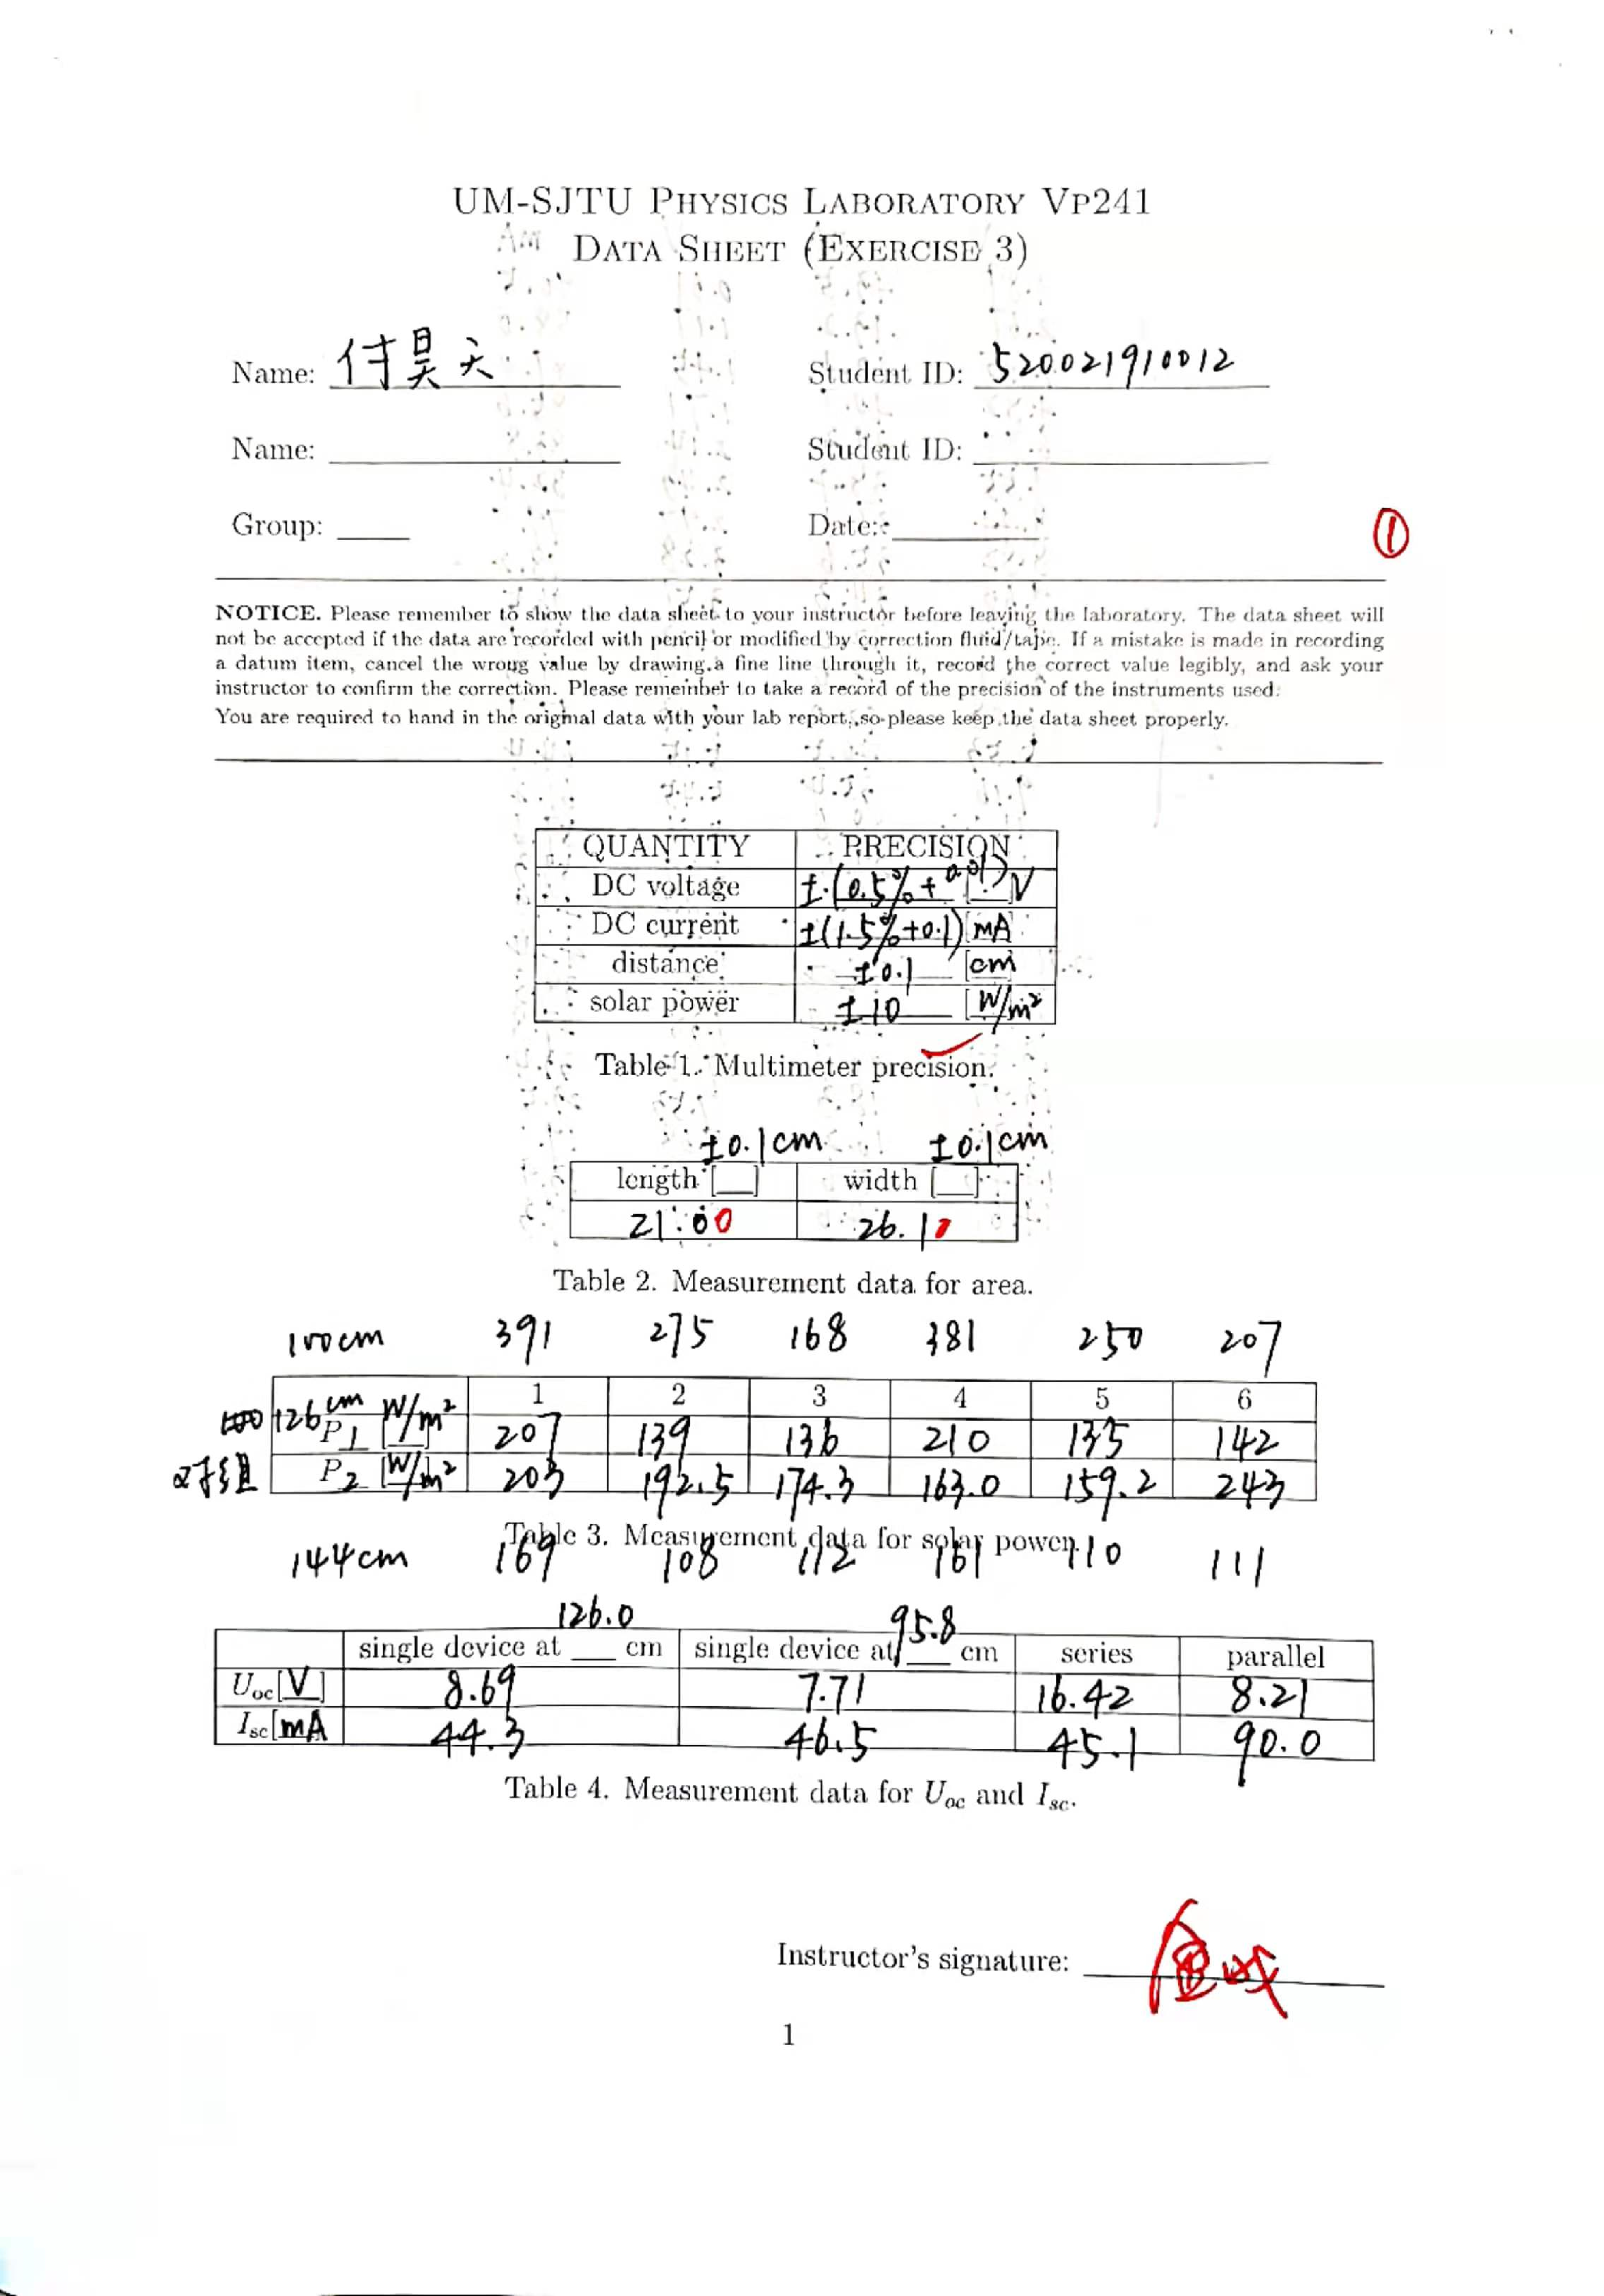
\includepdf{data_sheet_1.pdf}
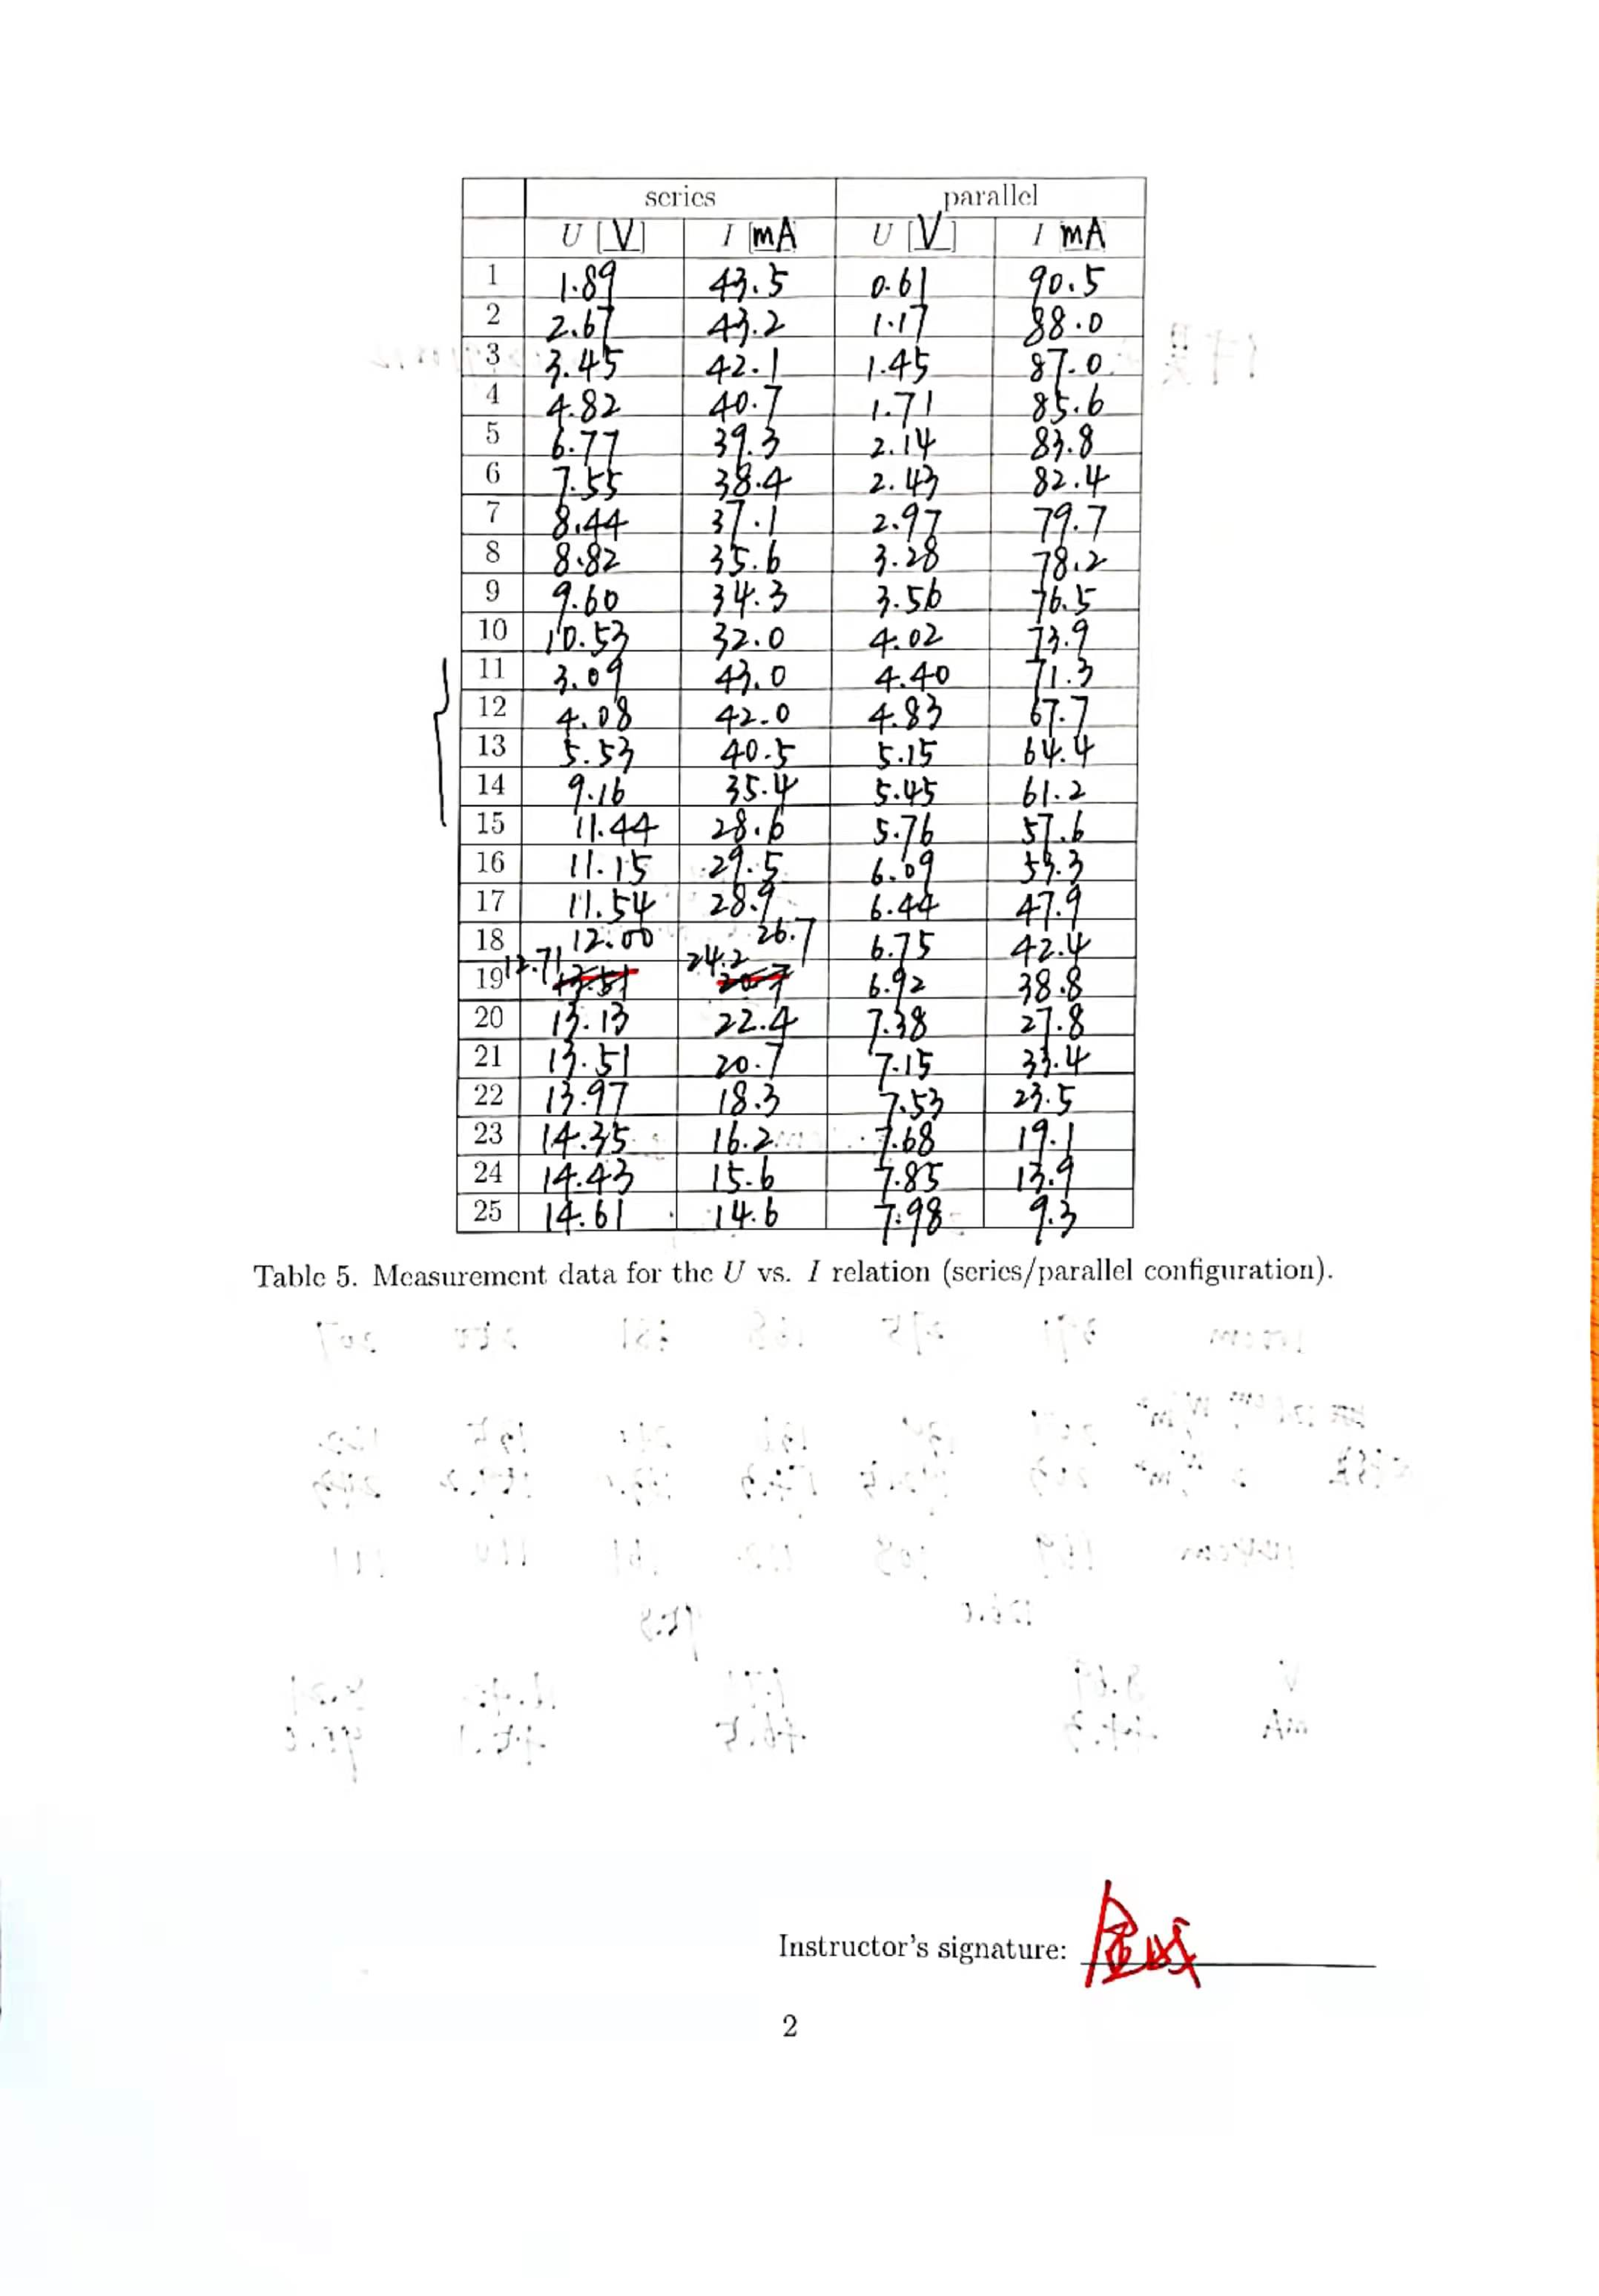
\includepdf{data_sheet_2.pdf}
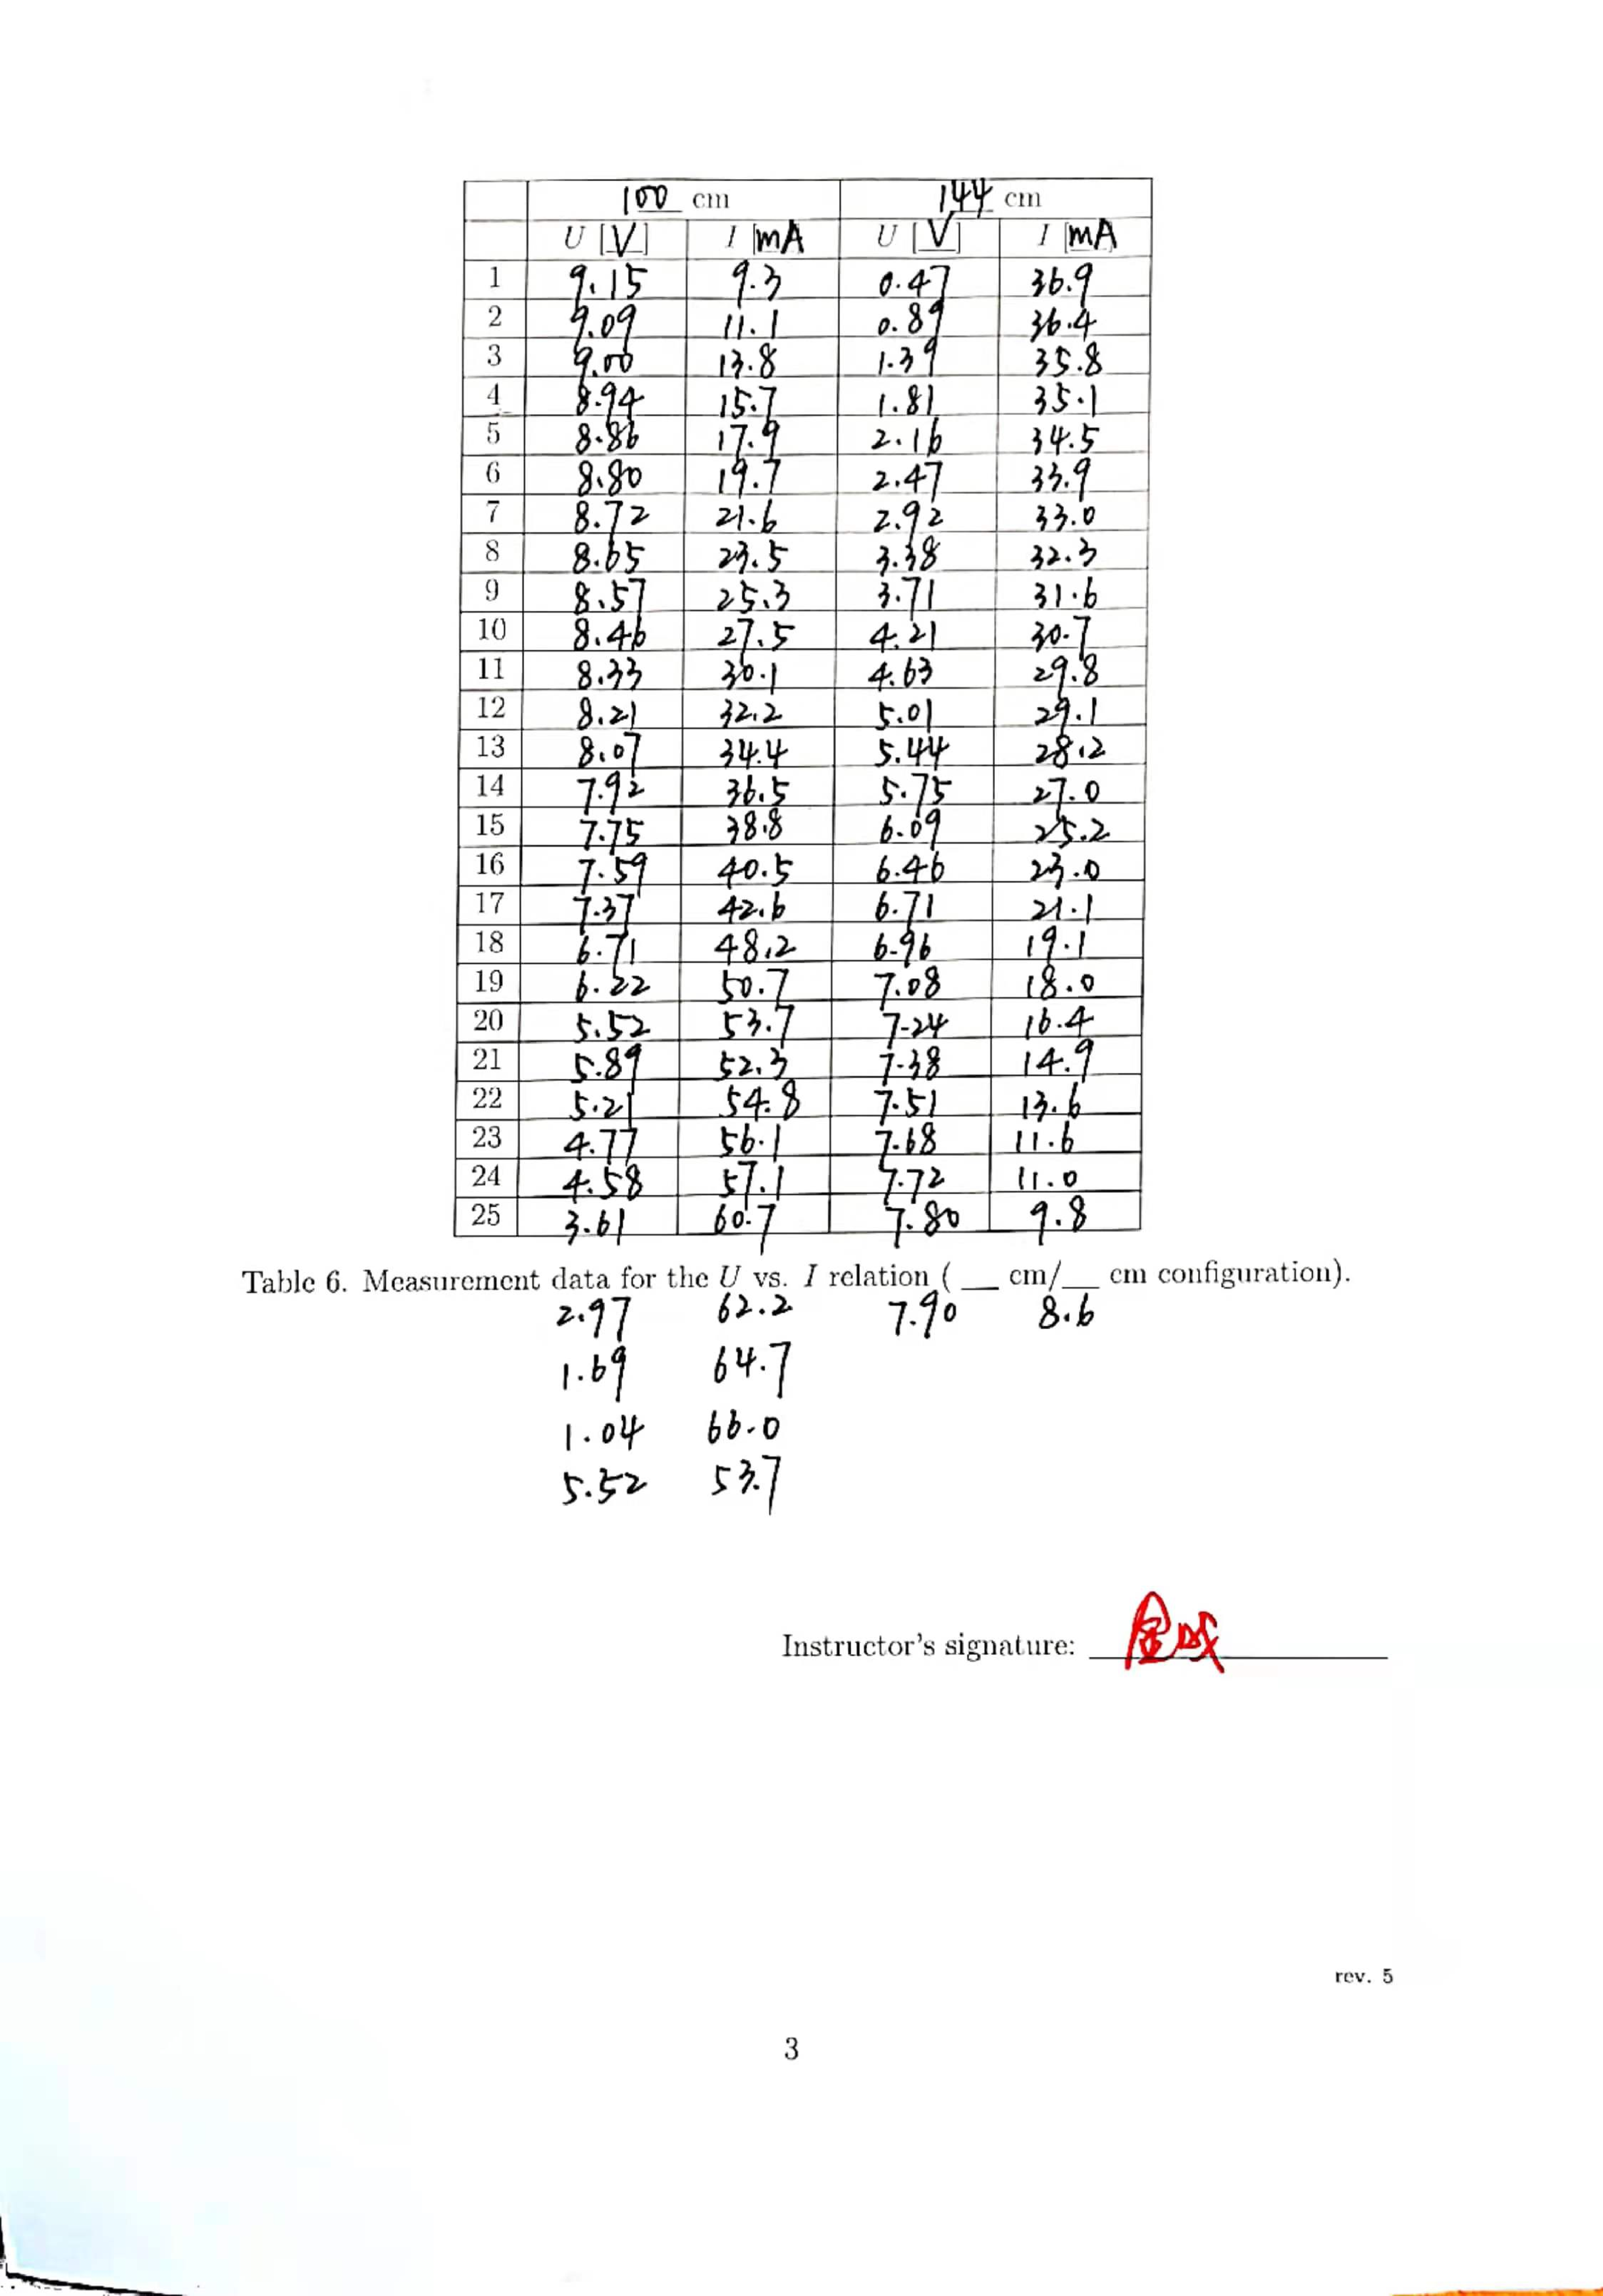
\includepdf{data_sheet_3.pdf}

\end{document}
